\def\modulename{pcp}
\def\solutions{false}
\RequirePackage[utf8]{course}
\pcp

\usepackage{Cdefs}

\usepackage[utf8]{inputenc}

\usepackage{listings}

%\newenvironment{flist}{\begin{itemize}}{\end{itemize}}
\newcommand{\itemex}[1]{ & \#1 \\ }

\newenvironment{petitexemple}{
  \begin{tabular}{l@{\hspace*{0.1\linewidth}}p{0.8\linewidth}}
    \mbox{\bf Exemple:} 
}{\end{tabular}}

\newenvironment{petitsexemples}{
  \begin{tabular}{l@{\hspace*{0.1\linewidth}}p{0.8\linewidth}}
    \mbox{\bf Exemples:} 
}{\end{tabular}}


\newenvironment{consigne}[1]%
{\begin{center}\begin{minipage}{13cm}%
{\large #1}\par}%
{\end{minipage}\end{center}\relax}
\def\Question#1#2{\question{}\textbf{(#2)} #1}


\def\nicefrac#1#2{\ensuremath{#1/#2}}
\newcommand{\matrice}[3]{\ensuremath{{({#1}_{i,j})}_{\hspace*{-1ex}\begin{array}{c}\scriptscriptstyle 1\le i \le  #2\\[-1ex]\scriptscriptstyle 1 \le j \le #3\end{array}}}}

\setlength{\itemsep}{0pt}


\usepackage{caption}
\usepackage{subcaption}
\usepackage{units}


\usepackage{tikz}
\usetikzlibrary{arrows}

\tikzset{
  treenode/.style = {align=center, inner sep=0pt, text centered,
    font=\sffamily},
  arn_n/.style = {treenode, circle, white, font=\sffamily\bfseries, draw
=black,
    fill=black, text width=1.5em},
  arn_r/.style = {treenode, circle, red, draw=red, 
    text width=1.5em, very thick},
  arn_x/.style = {treenode, rectangle, draw=black,
    minimum width=0.5em, minimum height=0.5em}
}
\begin{document}

\exo{Algorithmique}

Pour une formation, nous disposons de ta\-bleaux de notes (de type
\emph{float}) contenant les moyennes des {\'e}tudiants
(num{\'e}rot{\'e}s {\`a} partir de $0$) et d'un tableau contenant le
nom complet de chaque {\'e}tudiant Par exemple, si le nom complet d'un
{\'e}tudiant est \texttt{Bernard Pivot}, qu'il a eu \texttt{12.5} en
math{\'e}matiques, et que son num{\'e}ro est 5:
\begin{flist}
\item la cinqui{\`e}me case du tableau de noms vaut \cstring{Bernard
    Pivot}, et
\item la cinqui{\`e}me case du tableau de notes correspondant aux
  math{\'e}matiques vaut \texttt{12.5}.
\end{flist}

\begin{center}
  \fbox{\begin{minipage}{.9\linewidth} Dans les questions suivantes,
      pour chaque fonction, et dans cet ordre:
    \begin{flist}
    \item Indiquez le profil de la fonction que vous allez {\'e}crire ;
    \item D{\'e}crivez en une phrase ses arguments et la valeur qu'elle
      retourne ;
    \item {\'E}crivez la fonction en C.
    \end{flist}
  \end{minipage}}
\end{center}


\question (1 pt) Quel est le type d'un tableau de noms ?

\question (2 pts) {\'E}crire une fonction \cfun{Affiche} qui prend en
entr{\'e}e un tableau de notes, un tableau de noms, et le nombre
d'{\'e}tu\-diants, et qui affiche les notes (avec l'{\'e}tudiant
correspondant) avec une pr{\'e}cision de 3 chiffres apr{\`e}s la
virgule.

\question (2 pts) {\'E}crire une fonction \cfun{Moyenne} qui prend en
entr{\'e}e un tableau de \cfloat repr{\'e}sentant les notes d'une
mati{\`e}re, le nombre d'{\'e}tu\-diants, et qui retourne la moyenne
de la classe pour la mati{\`e}re repr{\'e}sent{\'e}e par le tableau.


\question (2 pts) {\'E}crire une fonction \cfun{Major} qui, a partir
d'un tableau de notes, retourne le num{\'e}ro de l'{\'e}tudiant ayant
obtenu la meilleure note

\question (2 pts) Faire une fonction \cfun{Passe} qui prend en
entr{\'e}e les un tableau de notes et le nombre d'{\'e}tudiants, et
rend en sortie un tableau $t$ d'entiers avec $t[i]=1$ si
l'{\'e}l{\`e}ve de num{\'e}ro $i$ a la moyenne, et $t[i]=0$ sinon.

\question (4 pts) {\'E}crire une fonction \cfun{MiseAJour} qui prend un num{\'e}ro
  d'{\'e}tudiant et propose de mettre {\`a} jour la moyenne de cet {\'e}tudiant
  dans une mati{\`e}re. Pour cela, cette fonction:
  \begin{flist}
  \item affiche la note courante courante de l'{\'e}tudiant dans cette
    mati{\`e}re;
  \item demande une nouvelle note, puis :
    \begin{flist}
    \item si l'utilisateur rentre une note, la fonction met {\`a} jour la
      note de l'{\'e}tudiant ;
    \item sinon, l'ancienne note est inchang{\'e}e.
    \end{flist}
  \end{flist}


\newpage


\exo{Bicha{\^\i}nes}

On fixe la structure suivante pour contenir les couples
($\langle$clef$\rangle$,$\langle$valeur$\rangle$).
\begin{lstlisting}
  struct bichaine_s {
  int l1 ;
  int l2 ;
  char * clef ;
  char * valeur ;
};
\end{lstlisting}


\question (1 pt) D{\'e}finir le type \texttt{bichaine} des pointeurs vers
une structure \texttt{bichaine\_s}.

\question (2 pts) {\'E}crire une fonction \texttt{nouvelle\_bichaine} qui
prend en entr{\'e}e 2 cha{\^\i}nes de caract{\`e}res et leur longueur, et rend une
valeur de type \texttt{bichaine}.

\question (2 pts) {\'E}crire deux fonctions \texttt{clef} et
\texttt{valeur} qui prennent en entr{\'e}e une bicha{\^\i}ne et rendent
respectivement sa clef et sa valeur.

\question (1 pt) {\'E}crire une fonction qui affiche une bicha{\^\i}ne dans le
format \texttt{$\langle$clef$\rangle$: $\langle$valeur$\rangle$} suivi
dans cet ordre par les deux caract{\`e}res \verb+\n+ et \verb+\f+.

\question (3 pts) {\'E}crire une fonction qui prend en entr{\'e}e
\textbf{les adresses} de 2 valeurs de type \texttt{bichaine}, et rend 
un entier positif, nul, ou n{\'e}gatif si la premi{\`e}re est plus grande,
{\'e}gale, ou plus petite que la seconde. Pour comparer 2 bichaines:
\begin{itemize}
\item si les deux sont \texttt{NULL}, elles sont {\'e}gales ;
\item si une seule des deux est \texttt{NULL}, c'est la plus
  grande ;
\item si aucune n'est nulle, alors le r{\'e}sultat est celui de la
  comparaison de leur \textbf{clef}.
\end{itemize}
En particulier, on note que si deux bicha{\^\i}nes ont la m{\^e}me clef, mais
des valeurs diff{\'e}rentes, elles seront consid{\'e}r{\'e}es comme {\'e}gales.



\newpage

\exo{Calcul de majorit{\'e} (14 pts)}

\begin{quotation}
  \sl Lors de l'ouverture de fichiers, il est demandé de faire
  attention aux cas possibles d'erreur.
\end{quotation}

  Un \emph{automate cellulaire unidimensionnel born{\'e}} est
  d{\'e}fini par un tableau fini de \emph{cellules}. Chaque \emph{cellule}
  est d{\'e}finie par un {\'e}tat. Cet automate cellulaire \emph{{\'e}volue} suivant une
  \emph{fonction de transition} qui indique comment chaque cellule doit 
  {\'e}voluer en regardant son {\'e}tat et celui de ses voisines.

  Cet exercice porte sur le probl{\`e}me de recherche de majorit{\'e} avec un
  automate cellulaire unidimensionnel born{\'e}. Les {\'e}tats ne peuvent
  {\^e}tre que \texttt{oui} ou \texttt{non}, et on veut faire {\'e}voluer un
  automate pour que toutes ses cellules soient {\`a} \texttt{oui} s'il y a
  une majorit{\'e} de oui-s, ou \texttt{non} s'il y a une majorit{\'e} de non-s.

  Une solution (qui ne marche pas toujours, car le probl{\`e}me n'a pas de
  solutions en g{\'e}n{\'e}ral) consiste {\`a} utiliser la fonction de transition
  suivante:
  \begin{itemize}
  \item Si l'{\'e}tat de la cellule $i$ est \texttt{oui}, alors le nouvel 
  {\'e}tat est celui de la majorit{\'e} entre cette cellule, celle {\`a} 
  l'adresse $i-1$, et celle {\`a} l'indice $i-3$ ;
  \item Si l'{\'e}tat de la cellule $i$ est \texttt{non}, alors le nouvel 
  {\'e}tat est celui de la majorit{\'e} entre cette cellule, celle {\`a} 
  l'adresse $i+1$, et celle {\`a} l'indice $i+3$.
  \end{itemize}
  Les indices dans le tableau sont modulo $n$, le nombre de cellules 
  dans l'automate cellulaire unidimensionnel.

\vspace*{1em}

\question (1 pt) Pour simplifier le calcul de majorit{\'e}, on veut d{\'e}finir
une cellule comme pouvant avoir 2 {\'e}tats, \texttt{oui} et
\texttt{non}, avec \texttt{oui} qui vaut $1$, et \texttt{non} qui vaut
$-1$. D{\'e}finir le type \texttt{cellule} des cellules.


\question (1 pt) On d{\'e}finit maintenant les automates comme des couples ayant:
\begin{enumerate}
\item un tableau de cellules;
\item un entier $n$ indiquant le nombre de cellules dans l'automate.
\end{enumerate}.
D{\'e}finir la structure \texttt{automate\_s} de ces couples, ainsi que le type 
\texttt{automate} des pointeurs vers ces structures.


\question (2 pts) {\'E}crire une fonction \url{nouvel_automate} qui
prend en entr{\'e}e un entier $n$, et qui rend un automate pouvant
contenir $n$ cellules. \textit{Il n'est pas demand{\'e} d'initialiser la
  valeur de ces cellules.}


Pour simplifier le traitement des erreurs, dans la suite, vous pouvez
utiliser la fonction \emph{erreur}, qui s'utilise exactement comme la
fonction \emph{printf}, mais termine le programme imm{\'e}diatement quand
elle est appel{\'e}e. Par exemple:

\begin{Ccode}
  \ctab \cif ( ( \emph{f} $=$ \url{fopen}( \emph{fichier}, \texttt{"r"}) ) $==$ \texttt{NULL} )
  \ctab\hspace*{2em}  \url{erreur} ( \texttt{"Impossible d'ouvrir le fichier \%s en lecture, fin."} , \emph{fichier} ) ;
\end{Ccode}



\question (2 pts) {\'E}crire une fonction \url{lire_etat_initial} qui
prend en entr{\'e}e le \emph{nom} d'un fichier, et qui:
\begin{itemize}
\item ouvre ce fichier en lecture ;
\item lit un entier $n$, qui sera la taille de l'automate, dans ce fichier;
\item construit un automate ayant $n$ cellules ;
\item lit les $n$ valeurs de cellules stock{\'e}es dans le fichier 
(le caract{\`e}re \texttt{'.'} pour \texttt{non}, et le caract{\`e}re 
\texttt{'*'} pour \texttt{oui}, aucun autre caract{\`e}re n'est autoris{\'e}).
\item ferme le fichier.
\end{itemize}

\paragraph{Exemple.} On donne ci-dessous un fichier bien formatt{\'e} qui doit {\^e}tre lu sans erreurs:
\begin{verbatim}
30
...**.*.***..**..**...***..***
\end{verbatim}

\question (2 pts) {\'E}crire une fonction \url{ecrire_automate} qui
prend en entr{\'e}e un fichier ouvert en {\'e}criture (de type \texttt{FILE
*}) et un automate, et {\'e}crit les cellules de l'automate sur une ligne
de ce fichier.


\question (2 pts) {\'E}crire une fonction \url{vote} qui prend en entr{\'e}e
un automate $a$ et le num{\'e}ro $i$ d'une cellule de cet automate, et
renvoie le nouvel {\'e}tat pour la cellule $i$ de $a$. \textit{Rappel: 
l'op{\'e}rateur C \% calcule le ``modulo'': $7\% 5 == 2$  mais \(-3 \% 5 == -3\)}.




\question (1 pt) {\'E}crire une fonction \url{suivant} qui prend en
entr{\'e}e un automate et renvoie un nouvel automate contenant
l'évolution de toutes les cellules de l'automate en argument de la fonction.


\question (2 pts) {\'E}crire une fonction \url{evolution} qui prend en
entr{\'e}e le nom d'un fichier et:
\begin{enumerate}
\item lit l'automate $a$ qui est d{\'e}finit au d{\'e}but de ce fichier;
\item r{\'e}-ouvre ce fichier en \emph{{\'e}criture en ajout};
\item calcule les 100 {\'e}volutions de l'automate $a$, et {\'e}crit dans 
le fichier tous les automates calcul{\'e}s;
\item referme le fichier.
\end{enumerate}
Comme pr{\'e}c{\'e}demment, il est demand{\'e} de faire tr{\`e}s attention {\`a} tous les
cas possibles d'erreur.


\question (1 pt) {\'E}crire la fonction \url{main} d'un programme qui
prend en entr{\'e}e exactement 1 argument, qui est le nom d'un fichier. Le
programme doit compl{\'e}ter le fichier en {\'e}crivant les 100 automates qui
suivent celui qui est d{\'e}j{\`a} dans le fichier.

\paragraph{Exemple.} {\`A} la fin, le fichier a la forme suivante (les
derni{\`e}res lignes sont enlev{\'e}es car toutes identiques):

\begin{verbatim}
30
...**.*.***..**..**...***..***
....****.**..**..**..*.**.****
...*.***.**..**..**.**..******
..*.*.**.**..**..**.**.*******
.***...*.**..**..**.**********
****..*...*..**..*************
****..*......**.**************
****..*.......****************
****..*......*.***************
****..*.....*.*.**************
****..*....*.*.*.*************
****..*...*.*.*.*.************
****..*..*.*.*.*.*.***********
****..*.***.*.*.*.*.**********
****.***.*****.*.*.*.*********
*****************.*.*.********
********************.*.*******
***********************.******
******************************
******************************
\end{verbatim}



\newpage


\exo{Calendrier (9pts)}

Dans cette partie, on mod{\'e}lise une date par un triplet
jour-mois-ann{\'e}e.

\question (1pt) On veut mod{\'e}liser les mois en utilisant dans le programme
les noms des mois (janvier, f{\'e}vrier, \ldots) plut{\^o}t que des entiers.
Donnez la d{\'e}claration C {\`a} {\'e}crire.

\begin{solution}
  \begin{Ccode}
    \ctab{}enum \cvar{mois} \lb janvier = 1 , fevrier , mars , avril , 
    \ctab{} mai , juin , juillet , aout , septembre , octobre, 
    \ctab{}novembre , decembre \rb ;
  \end{Ccode}
\end{solution}


\question (0.5pt) Donnez la d{\'e}finition de structure permettant de
mod{\'e}liser une date.

\question (1pt) {\'E}crire une fonction \cfun{date} qui prend en entr{\'e}e
un jour, un mois, et une ann{\'e}e,  et qui rend une date.

\begin{solution}
  \begin{Ccode}
    \ctab{}\cstruct \ctype{date\_std} *
    \ctab{}\cfun{date\_std} ( \cint \cvar{jour} , enum \cvar{mois} \cvar{mois} , \cint \cvar{an} )
    \ctab{}\lb
    \ctab{}  \cstruct \ctype{date\_std} * \cvar{res} ;
    \ctab{}  \cvar{res} = ( \cstruct \ctype{date\_std} * ) \cfun{malloc} ( \cfun{sizeof} ( \cstruct \ctype{date\_std} ) ) ;
    \ctab{}  \cvar{res}\ensuremath{\rightarrow}\cvar{jour} = \cvar{jour} ;
    \ctab{}  \cvar{res}\ensuremath{\rightarrow}\cvar{mois} = \cvar{mois} ;
    \ctab{}  \cvar{res}\ensuremath{\rightarrow}\cvar{an} = \cvar{an} ;
    \ctab{}  \creturn \cvar{res} ;
    \ctab{}\rb
  \end{Ccode}
\end{solution}

\question (1pt) {\'E}crire une fonction affichant une date.

\question (0.5pt) {\'E}crire une fonction \cfun{bissextile} qui rend vrai si
l'ann{\'e}e donn{\'e}e en argument est bissextile, et faux sinon.

\hspace*{5em}\parbox{0.8\linewidth}{\underline{Rappel:} une ann{\'e}e
  $n$ est bissextile si, et seulement si, $n$ est divisible par 400 ou
  si $n$ est divisible par 4 mais pas par 100.}

\begin{solution}
  \begin{Ccode}
\ctab{}\cint
\ctab{}\cfun{bissextile} ( \cint \cvar{annee} ) 
\ctab{}\lb
\ctab{}  \creturn ( \cvar{annee} \% 4 == 0 ) \&\& ( ( \cvar{annee} \% 100 != 0 ) || ( \cvar{annee} \% 400 == 0 ) ) ;
\ctab{}\rb
  \end{Ccode}
\end{solution}

\question (1pt) {\'E}crire une fonction \cfun{nb\_jours} qui prend en
entr{\'e}e une date et rend le nombre de jours du mois de cette date.


\begin{petitsexemples}
\itemex{ \cfun{nb\_jours}(10/01/2012) = 31}
\itemex{ \cfun{nb\_jours}(5/11/2011) = 30}
\end{petitsexemples}

\begin{solution}
  \begin{Ccode}
    \ctab{}\cint 
    \ctab{}\cfun{\cvar{nb\_jours}} ( \cstruct \ctype{date} * \cvar{d} )
    \ctab{}\lb
    \ctab{}    \cfun{switch} ( \cvar{d}\ensuremath{\rightarrow}\cvar{mois} )
    \ctab{}      \lb
    \ctab{}      case janvier:
    \ctab{}      case mars:
    \ctab{}      case mai:
    \ctab{}      case juillet:
    \ctab{}      case aout:
    \ctab{}      case octobre:
    \ctab{}      case decembre:
    \ctab{}	\creturn  31 ;
    \ctab{}      case 4:
    \ctab{}      case 6:
    \ctab{}      case 9:
    \ctab{}      case 11:
    \ctab{}	\creturn 30 ;
    \ctab{}      default: /* case 2: */
    \ctab{}      \cif ( \cfun{bissextile} ( \cvar{d}\ensuremath{\rightarrow}\cvar{an} ) )
    \ctab{}	\creturn 29 ;
    \ctab{}      \celse
    \ctab{}	\creturn 28 ;
    \ctab{}    \rb
    \ctab{}\rb
  \end{Ccode}
\end{solution}

\question (3pts) {\'E}crire une fonction \cfun{jour\_suivant} qui change
la date en argument en la date du jour suivant.

\hspace*{5em}\parbox{0.8\linewidth}{\underline{Indication:} une
  possibilit{\'e} est d'{\'e}crire 3 fonctions changeant la date en,
  respectivement, le premier janvier de l'ann{\'e}e suivant, le premier
  jour du mois suivant, et finalement le jour suivant.}

\begin{petitsexemples}
  \itemex{ \cfun{jour\_suivant}(31/12/2011) = 01/01/2012}
  \itemex{ \cfun{jour\_suivant}(28/02/2012) = 29/02/2012}
\end{petitsexemples}

\begin{solution}
  \begin{Ccode}
    \ctab{}\cstruct \ctype{date} *
    \ctab{}\cfun{\cvar{an}\_suivant} ( \cstruct \ctype{date} * \cvar{d} )
    \ctab{}\lb
    \ctab{}  \cif ( \cvar{d} == \cvar{NULL} )
    \ctab{}    \creturn \cvar{NULL} ;
    \ctab{}
    \ctab{}  \cvar{d}\ensuremath{\rightarrow}\cvar{mois} = janvier ;
    \ctab{}  \cvar{d}\ensuremath{\rightarrow}\cvar{an} = \cvar{d}\ensuremath{\rightarrow}\cvar{an} + 1 ;
    \ctab{}  \creturn \cvar{d} ;
    \ctab{}\rb
    \ctab{}
    \ctab{}\cstruct \ctype{date} *
    \ctab{}\cfun{\cvar{mois}\_suivant} ( \cstruct \ctype{date} * \cvar{d} )
    \ctab{}\lb
    \ctab{}  \cif ( \cvar{d} == \cvar{NULL} )
    \ctab{}    \creturn \cvar{NULL} ;
    \ctab{}
    \ctab{}  \cvar{d}\ensuremath{\rightarrow}\cvar{jour} = 1 ;
    \ctab{}  \cif ( \cvar{d}\ensuremath{\rightarrow}\cvar{mois} < decembre ) 
    \ctab{}    \cvar{d}\ensuremath{\rightarrow}\cvar{mois} = \cvar{mois} + 1 ;
    \ctab{}  \celse
    \ctab{}    \cvar{d} =  \cfun{\cvar{an}\_suivant} ( \cvar{d} ) ;
    \ctab{}  \creturn \cvar{d} ;
    \ctab{}\rb
    \ctab{}
    \ctab{}\cstruct \ctype{date} *
    \ctab{}\cfun{\cvar{jour}\_suivant} ( \cstruct \ctype{date} * \cvar{d} )
    \ctab{}\lb
    \ctab{}  \cif ( \cvar{d} == \cvar{NULL} )
    \ctab{}    \creturn \cvar{NULL} ;
    \ctab{}
    \ctab{}  \cif ( \cvar{d}\ensuremath{\rightarrow}\cvar{jour} < \cfun{\cvar{nb\_jours}} ( \cvar{d} ) )
    \ctab{}    \cvar{d}\ensuremath{\rightarrow}\cvar{jour} = \cvar{d}\ensuremath{\rightarrow}\cvar{jour} + 1 ;
    \ctab{}  \celse
    \ctab{}   \cvar{d} = \cfun{\cvar{mois}\_suivant} ( \cvar{d} ) ;
    \ctab{}  \creturn \cvar{d} ;
    \ctab{}\rb
  \end{Ccode}
\end{solution}

\question (1pt) {\'E}crire une fonction \cfun{avance} qui change une date
en celle de $n$ jours plus tard.

\begin{petitexemple}
  \itemex{\cfun{avance}(27/01/2012 , 5 ) = 01/02/2012}
\end{petitexemple}

\begin{solution}
  \begin{Ccode}
    \ctab{}\cstruct \ctype{date} * \ctab{}\cfun{avance} ( \cstruct
    \ctype{date} * \cvar{d} , \cint \cvar{n} ) \ctab{}\lb \ctab{} \cif
    ( \cvar{d} == \cvar{NULL} ) \ctab{} \creturn \cvar{NULL} ; \ctab{}
    \cif ( \cvar{n} == 0 ) \ctab{} \creturn \cvar{d} ; \ctab{} \ctab{}
    \creturn \cfun{avance} ( \cfun{\cvar{jour}\_suivant} ( \cvar{d} )
    , \cvar{n} - 1 ) ; \ctab{}\rb
  \end{Ccode}
\end{solution}


\newpage


\exo{Calendrier (bis) (5pts)}

Cette partie est plus complexe que
les pr{\'e}c{\'e}dentes ; il est d{\'e}conseill{\'e} de l'aborder avant d'avoir termin{\'e}
ce qui pr{\'e}c{\`e}de. On cherche {\`a} nouveau {\`a} mod{\'e}liser des dates, mais cette
fois dans le format jour-semaine-an:
\begin{flist}
\item le dimanche de la semaine 0 de 2012 est le 01/01/2012 ;
\item le mercredi de la semaine 2 de 2012 est le 10/01/2012 ;
\item pour plus d'exemples, voir les deux calendriers en annexe.
\end{flist}
Chaque ann{\'e}e est divis{\'e}e en 53 ou 54 semaines, dont une ou deux
peuvent {\^e}tre incompl{\`e}tes. Une semaine commence soit un lundi, soit le
premier janvier (semaine 0), et se termine soit le dimanche, soit le
31 d{\'e}cembre (semaine 52).  Une ann{\'e}e normale dure $52\times 7 + 1$
jours, et une ann{\'e}e bissextile dure $52 \times 7 + 2$ jours. Dans les
questions suivantes, il est conseill{\'e} de d{\'e}finir des fonctions
auxiliaires pour faire les calculs. Il est possible de r{\'e}utiliser les
fonctions de l'exercice \textsc{II}.

\question (1pt) Donnez les types de donn{\'e}es que vous allez utiliser.

\question (2pts) {\'E}crire une fonction rendant la date du jour de l'an
d'une ann{\'e}e $n$.

\question (2pts) {\'E}crire deux fonctions transformant une date
jour-mois-an en une date jour-semaine-an et r{\'e}ciproquement.


\newpage

\exo{Championnat}

Le but de cet exercice est de mod{\'e}liser des championnats, c'est-{\`a}-dire
des matchs aller-retour entre des {\'e}quipes de telle sorte que chaque
{\'e}quipe rencontre deux fois chaque autre {\'e}quipe, une fois {\`a} domicile,
une fois {\`a} l'ext{\'e}rieur.


\question (1pt) {\'E}crire une fonction qui demande un nom d'{\'e}quipe (une
cha{\^\i}ne de caract{\`e}res) {\`a} l'utilisateur et renvoie cette cha{\^\i}ne de
caract{\`e}res. La cha{\^\i}ne de caract{\`e}res dans laquelle la fonction doit
stocker le nom de l'{\'e}quipe est pass{\'e}e en argument.

\question (2pts) On veut avoir une structure \ctype{championnat} qui
contient le nombre (un entier) et les noms des {\'e}quipes (des cha{\^\i}nes de
caract{\`e}res), et la longueur maximale (un entier) du nom d'une
{\'e}quipe. Donnez la d{\'e}claration de la structure \ctype{championnat}.

Une \emph{rencontre} est mod{\'e}lis{\'e}e par 4 entiers \cvar{equipe1},
\cvar{equipe2}, \cvar{score1}, \cvar{score2} qui repr{\'e}sentent:
\begin{itemize}
\item l'indice de l'{\'e}quipe 1 dans le tableau du championnat;
\item l'indice de l'{\'e}quipe 2 dans le tableau du championnat;
\item le score de l'{\'e}quipe 1 dans le match;
\item le score de l'{\'e}quipe 2 dans le match;
\end{itemize}
Les scores sont {\`a} $-1$ tant que le match n'est pas jou{\'e}.

\question (1pt) Donnez la d{\'e}claration de la structure
\ctype{rencontre} en fonction de ces donn{\'e}es.

\question (3pts) {\'E}crire une fonction qui demande {\`a} l'utilisateur:
\begin{itemize}
\item un nombre d'{\'e}quipes;
\item la taille maximale du nom d'une {\'e}quipe;
\item puis les noms de toutes les {\'e}quipes du championnant un par un;
\end{itemize}
et qui renvoie un \ctype{championnat} repr{\'e}sentant ces informations.

\question (2pts) {\'E}crire une fonction qui prend en entr{\'e}e une variable
de type \ctype{championnat} et une variable de type \ctype{rencontre} et
qui affiche le r{\'e}sultat de la rencontre dans le format:
\begin{center}
  \texttt{<nom \'Equipe1> <score1> -- <score2> <nom \'Equipe2>}
\end{center}
Par exemple:
\begin{center}
  \texttt{Stade Toulousain 18 -- 15 RC Toulon}
\end{center}

\question (3pts) {\'E}crire une fonction qui prend en entr{\'e}e un
championnat, et rend un tableau de rencontres entre les {\'e}quipes de ce
championnat dans lequel deux {\'e}quipes diff{\'e}rentes se rencontrent
exactement 2 fois. Les scores des rencontres seront initialis{\'e}s {\`a} $-1$.



\newpage

\exo{Correction d'un programme C}

\question (5 pts) Corriger le programme suivant pour qu'il affiche le maximum
  de 3 entiers (r{\'e}pondre sur le sujet)

\begin{Ccode}
\ctab{}\cinclude{\syslib{stdio}} 
\ctab{}\cint \cfun{main} (\cint \cvar{argc}, \cchar *\cvar{argv}[])\lb
\ctab{}  \cint \cvar{nb1},\cvar{nb2},\cvar{nb3},\cvar{n1},\cvar{n2},*
\cvar{n3},
\ctab{}  \cint \cvar{max};
\ctab{}  \ccomment{Demande des nombres} 
\ctab{}  \cfun{printf}(\cstring{Donner votre premier nombre : });
\ctab{}  \cdo \{ \cvar{nb1} = \cfun{scanf}(\cstring{\%f},\&\cvar{n1}) ; 
\cwhile (\cfun{getchar}() != '\n' ) ; \} \cwhile ( \cvar{n1} == 0 );    
\ctab{}  \cfun{printf}(\cstring{Donner votre deuxieme nombre : });
\ctab{}  \cdo \{ \cvar{nb2} = \cfun{scanf}(\cstring{\%d},\&\cvar{n2}) ; 
\cwhile (\cfun{getchar}() != '\n' ) ; \} \cwhile ( \cvar{nb2} = 0 );
\ctab{}  \cfun{printf}(\cstring{Donner votre troisieme nombre : });     
   
\ctab{}  \cdo \{ \cvar{nb3} = \cfun{scanf}(\cstring{\%s},\cvar{n3}) ; 
\cwhile (\cfun{getchar}() != '\n' ) ; \} \cwhile ( \cvar{nb3} = 0 );      
                         
\ctab{}  \cif (\cvar{n1}>\cvar{n2}) ;                                   
    
\ctab{}    \lb
\ctab{}      \cvar{max} = \cvar{n1};
\ctab{}      \cif (\cvar{n3} > \cvar{max} )
\ctab{}          \hspace*{2em}\cvar{max} = *\cvar{n3};
\ctab{}    \rb
\ctab{}  \celse
\ctab{}    \lb
\ctab{}      \cvar{max} = \cvar{n2};
\ctab{}      \cif (\cvar{n3} > \cvar{max} )
\ctab{}        \lb
\ctab{}          \cvar{max} = *\cvar{n3}
\ctab{}        \rb 
\ctab{}    \rb
\ctab{}  \cfun{printf} (\cstring{Le maximum de \%d \%d \%d est \%d \n},
\&\cvar{n1},\&\cvar{n2},\cvar{n3},\&\cvar{max}); 
\ctab{}  \creturn 0;
\ctab{}\rb
\end{Ccode}



\newpage


\exo{Algorithmique}

On organise des {\'e}lections pour lesquelles il y a $C$ candidats et $S$
{\'E}tats. Les r{\'e}sultats des candidats dans chaque {\'E}tat sont stock{\'e}s dans
un tableau. S'il y a $C=3$ candidats et $S=2$
{\'e}tats, ce tableau contient par exemple:
\begin{center}
  \begin{tabular}{|l|c|c|c|}
    \hline
    {\'e}tat$\bslash$candidat & 0 & 1 & 2 \\
    \hline
    0 & 150 & 200 & 10 \\
    \hline
    1 & 33 & 120 & 3 \\
    \hline
  \end{tabular}
\end{center}


\question (2 pts) {\'E}crire une fonction \cfun{initialisation} qui prend en
  entr{\'e}e le nombre $C$ de candidats et le nombre $N$ d'{\'e}tats, et rend
  l'adresse d'un tableau pouvant stocker les
  r{\'e}sultats du vote pour une {\'e}lection {\`a} $C$ candidats et $S$ {\'e}tats.

\question (1 pt) {\'E}crire une fonction \cfun{affichageCandidatEtat} qui prend
  en entr{\'e}e le tableau stockant les r{\'e}sultats du vote, un num{\'e}ro de
  candidat $c$ et un num{\'e}ro d'{\'e}tat $s$ et qui affiche le nombre de voix
  obtenu par le candidat $c$ dans l'{\'e}tat $s$.

\question (1 pt) {\'E}crire une fonction \cfun{entreeCandidatEtat} qui prend en
  entr{\'e}e le tableau stockant les r{\'e}sultats du vote, un num{\'e}ro de
  candidat $c$ et un num{\'e}ro d'{\'e}tat $s$, qui demande {\`a} l'utilisateur le
  nombre de voix obtenu par le candidat $c$ dans l'{\'e}tat $s$, et qui
  met {\`a} jour le tableau de r{\'e}sultats.

\question (2 pts) {\'E}crire une fonction \cfun{totalVoixCandidat} qui rend le
  nombre total des voix obtenues par ce candidat.

\question (2 pts) {\'E}crire une fonction \cfun{totalVoix} qui rend le nombre
total de votes.


\question (2 pts) {\'E}crire une fonction \cfun{president} qui rend le candidat
  ayant remport{\'e} le plus d'{\'e}tats.



\newpage




\exo{Jeu de la vie}

Le \emph{jeu de la vie} est un jeu informatique qui se joue dans un
tableau {\`a} deux dimensions $n\times m$. Chaque case de ce tableau,
appel{\'e}e \emph{cellule}, est soit vivante, soit morte. Chaque cellule a
8 \emph{voisines} (dans les 8 directions nord, nord-ouest, ouest,
sud-ouest, sud, sud-est, est, nord-est). Les cellules au-del{\`a} des
bords sont toutes consid{\'e}r{\'e}es comme mortes. Un \emph{{\'e}tat} est un
tableau dans lequel chaque cellule est soit vivante, soit morte.

On passe de l'{\'e}tat courant {\`a} l'{\'e}tat suivant en examinant, pour
chaque cellule en dehors des bords, le nombre $k$ de voisines en
vie\,:
\begin{itemize}
\item s'il y en a 3, et que la cellule est morte, elle devient vivante\,;
\item s'il y en a 2 ou 3, et que la cellule est vivante, elle le reste\,;
\item Dans tous les autres cas, la cellule meurt.
\end{itemize}


\question (1 pt) D{\'e}clarer le type pour repr{\'e}sentant l'{\'e}tat des
cellules.

\question (1 pt) D{\'e}clarer un type pour repr{\'e}senter les tableaux dans
lesquels se jouent le jeu de la vie.

\question (1 pt) {\'E}crire un fonction prenant en entr{\'e}e deux entiers $n$
et $m$, et rendant un tableau pour le jeu de la vie dans lequel toutes
les cellules sont mortes.

\question (1 pt) {\'E}crire une fonction donnant le nombre de voisines
vivantes d'une cellule dans un tableau.


\question (3 pts) {\'E}crire une fonction prenant en entr{\'e}e un tableau
(ainsi qu'{\'e}ventuellement d'autres arguments) repr{\'e}sentant un {\'e}tat
courant, et rendant un tableau contenant l'{\'e}tat suivant.

\paragraph{Exemple.} Dans la suite d'{\'e}tats suivante, une cellule morte
est vide, une vivante est repr{\'e}sent{\'e}e par un V.
\def\morte{\phantom{V}} \def\vivante{V}
\begin{center}
\begin{tabular}[c]{|c|c|c|c|c|}
    \hline 
    \morte{}&\morte{}&\morte{}&\morte{}&\morte{}\\
    \hline 
    \morte{}&\vivante{}&\morte{}&\morte{}&\morte{}\\
    \hline 
    \morte{}&\vivante{}&\vivante{}&\vivante{}&\morte{}\\
    \hline 
    \morte{}&\morte{}&\morte{}&\vivante{}&\morte{}\\
    \hline 
    \morte{}&\morte{}&\morte{}&\morte{}&\morte{}\\
    \hline 
  \end{tabular} $\Rightarrow$ \begin{tabular}{|c|c|c|c|c|}
    \hline 
    \morte{}&\morte{}&\morte{}&\morte{}&\morte{}\\
    \hline 
    \morte{}&\vivante{}&\morte{}&\morte{}&\morte{}\\
    \hline 
    \morte{}&\vivante{}&\morte{}&\vivante{}&\morte{}\\
    \hline 
    \morte{}&\morte{}&\morte{}&\vivante{}&\morte{}\\
    \hline 
    \morte{}&\morte{}&\morte{}&\morte{}&\morte{}\\
    \hline 
  \end{tabular}
$\Rightarrow$
\begin{tabular}{|c|c|c|c|c|}
    \hline 
    \morte{}&\morte{}&\morte{}&\morte{}&\morte{}\\
    \hline 
    \morte{}&\morte{}&\vivante{}&\morte{}&\morte{}\\
    \hline 
    \morte{}&\morte{}&\morte{}&\morte{}&\morte{}\\
    \hline 
    \morte{}&\morte{}&\vivante{}&\morte{}&\morte{}\\
    \hline 
    \morte{}&\morte{}&\morte{}&\morte{}&\morte{}\\
    \hline 
  \end{tabular}
$\Rightarrow$
\begin{tabular}{|c|c|c|c|c|}
    \hline 
    \morte{}&\morte{}&\morte{}&\morte{}&\morte{}\\
    \hline 
    \morte{}&\morte{}&\morte{}&\morte{}&\morte{}\\
    \hline 
    \morte{}&\morte{}&\morte{}&\morte{}&\morte{}\\
    \hline 
    \morte{}&\morte{}&\morte{}&\morte{}&\morte{}\\
    \hline 
    \morte{}&\morte{}&\morte{}&\morte{}&\morte{}\\
    \hline 
  \end{tabular}

\end{center}



\newpage

\exo{Matrices (7 pts)}

Le but de cet exercice est d'{\'e}valuer les contributions individuelles
au projet. 

\question (1 pt) On d{\'e}finit une \emph{matrice enti{\`e}re} par: 
\begin{itemize}
\item un nombre de lignes et de colonnes ;
\item un tableau de lignes, chaque ligne {\'e}tant un tableau d'entiers.
\end{itemize}
D{\'e}finir le type \texttt{matrice} des pointeurs vers des structures C
repr{\'e}sentant des matrices enti{\`e}res.

\question (1 pt) {\'E}crire une fonction \textbf{matrice\_nulle} qui prend
en entr{\'e}e un nombre de lignes et de colonnes, et renvoie une matrice
dont tous les coefficients sont {\`a} $0$.

\question (2 pts) {\'E}crire une fonction qui renvoie le produit de 2
matrices, ou \texttt{NULL} si le produit n'est pas d{\'e}fini.

\question (1 pt) {\'E}crire une fonction \textbf{taille\_int} qui calcule le
nombre minimal de symboles {\`a} utiliser (y compris le \texttt{'-'} pour
les nombres n{\'e}gatifs) pour {\'e}crire un entier en base 10.

\question (1 pt) {\'E}crire une fonction \textbf{taille\_mat} qui renvoie
le maximum des tailles des entiers des coefficients d'une matrice
pass{\'e}e en argument.

\question (1 pt) Le \emph{mineur} $M_{i,j}$ d'une matrice carr{\'e}e $M$
de taille $n\times n$ est la matrice carr{\'e}e de taille $(n-1)\times
(n-1)$ construite {\`a} partir de $M$ en enlevant la $i${\`e}me ligne et la
$j${\`e}me colonne. En num{\'e}rotant les lignes et les colonnes {\`a} partir de
$0$, le \emph{d{\'e}terminant} de $M$ est not{\'e} $\vert M\vert$ et vaut:
$$
\vert M\vert = \Sigma_{j=0}^{n-1} (-1)^j \vert M_{0,j}\vert
$$
Donnez un ordre de grandeur, en fonction de $n$, pour le nombre de
calculs {\`a} effectuer dans une fonction calculant un d{\'e}terminant en
utilisant cette formule. \textit{Il n'y a pas de code C {\`a} {\'e}crire pour
  cette question !}





\newpage


\exo{Matrices (7pts)}

On revoit dans cette partie certaines fonctions {\'e}crites dans le
projet. On repr{\'e}sente les matrices avec des structures contenant:
\begin{flist}
\item un nombre \cvar{nb\_lig} de lignes ;
\item un nombre \cvar{nb\_col} de colonnes ;
\item un tableau \cvar{coefficients} de lignes, chaque ligne {\'e}tant un
  tableau de valeurs de type \cdouble.
\end{flist}

\question (1pt) Donnez la d{\'e}claration d'une structure \ctype{matrice}
correspondant {\`a} cette d{\'e}finition.
\begin{solution}
  \begin{Ccode}
    \ctab{}\cstruct \ctype{matrice} \lb
    \ctab{}  \cint \cvar{nb\_col} ;
    \ctab{}  \cint \cvar{nb\_lig} ;
    \ctab{}  \cdouble **coefficients ;
    \ctab{}\rb ;    
  \end{Ccode}
\end{solution}


\question (2pts) On veut n'avoir qu'une fonction, appel{\'e}e
\cfun{matrice}, qui cr{\'e}e des matrices en appelant la fonction
\cfun{malloc}. {\'E}crire cette fonction.
\begin{solution}
  $$
  \mbox{matrice}: \cint \times \cint \to \mbox{struct matrice *}
  $$
  \emph{matrice(i,j)} cr{\'e}e une matrice de $i$ lignes et $j$ colonnes.
  \begin{Ccode}
    \ctab{}\cstruct \ctype{matrice} *
\ctab{}\cfun{matrice} ( \cint \cvar{nb\_col} , \cint \cvar{nb\_lig} )
\ctab{}\lb
\ctab{}  \cint \cvar{\cvar{ligne}} ;
\ctab{}  \cstruct \ctype{matrice} * \cvar{\cvar{res}} ;
\ctab{}
\ctab{}  \cvar{\cvar{res}} = (\cstruct \ctype{matrice} *) \cfun{malloc} ( \cfun{sizeof} ( \cstruct \ctype{matrice} ) ) ;
\ctab{}
\ctab{}  \cvar{\cvar{res}} \ensuremath{\rightarrow} \cvar{nb\_col} = \cvar{nb\_col} ;
\ctab{}  \cvar{\cvar{res}} \ensuremath{\rightarrow} \cvar{nb\_lig} = \cvar{nb\_lig} ;
\ctab{}  \cvar{\cvar{res}} \ensuremath{\rightarrow} coefficients = ( \cdouble ** ) \cfun{malloc} ( \cvar{nb\_lig} * \cfun{sizeof} ( \cdouble * ) ) ;
\ctab{}
\ctab{}  \cfor ( \cvar{\cvar{ligne}} = 0 ; \cvar{\cvar{ligne}} < \cvar{nb\_lig} ; \cvar{\cvar{ligne}} ++ )
\ctab{}    \lb
\ctab{}      \cvar{\cvar{res}} \ensuremath{\rightarrow} coefficients[\cvar{\cvar{ligne}}] = ( \cdouble * ) \cfun{malloc} ( \cvar{nb\_col} * \cfun{sizeof} ( \cdouble ) ) ;
\ctab{}    \rb
\ctab{}
\ctab{}  \creturn \cvar{\cvar{res}} ;
\ctab{}\rb
  \end{Ccode}
\end{solution}

\question (2pts) {\'E}crire une fonction qui rend le r{\'e}sultat de
l'addition de deux matrices. V{\'e}rifiez que les matrices en entr{\'e}e 
sont bien d{\'e}finies et que l'addition des deux matrices en entr{\'e}e est
bien d{\'e}finie.

\begin{solution}
  $$
  \mbox{addition}:  \mbox{struct matrice *} \times \mbox{struct matrice *}  \to \mbox{struct matrice *}
  $$
  \emph{addition(a,b)} rend la matrice qui est le r{\'e}sultat de
  l'addition de $a$ et de $b$, ou \cvar{NULL} si $a=\cvar{NULL}$ ou
  $b=\cvar{NULL}$ ou $a$ et $b$ sont de tailles diff{\'e}rentes.
  \begin{Ccode}
\ctab{}\cstruct \ctype{matrice} *
\ctab{}\cfun{addition} ( \cstruct \ctype{matrice} * \cvar{\cvar{a}} , \cstruct \ctype{matrice} * \cvar{\cvar{b}} )
\ctab{}\lb
\ctab{}  \cstruct \ctype{matrice} * \cvar{c} ;
\ctab{}  \cint \cvar{\cvar{i}} , \cvar{\cvar{j}} ;
\ctab{}
\ctab{}  \cif ( ( \cvar{\cvar{a}} == \cvar{\cvar{\cvar{NULL}}} ) || ( \cvar{\cvar{b}} == \cvar{\cvar{\cvar{NULL}}} ) || 
\ctab{}       ( \cvar{\cvar{a}}\ensuremath{\rightarrow}\cvar{nb\_lig} != \cvar{\cvar{b}} \ensuremath{\rightarrow} \cvar{nb\_lig} ) || 
\ctab{}       ( \cvar{\cvar{a}}\ensuremath{\rightarrow}\cvar{nb\_col} != \cvar{\cvar{b}} \ensuremath{\rightarrow} \cvar{nb\_col} ) )
\ctab{}    \creturn \cvar{\cvar{\cvar{NULL}}} ;
\ctab{}
\ctab{}  \cvar{c} = \cfun{matrice} ( \cvar{\cvar{a}}\ensuremath{\rightarrow}\cvar{nb\_lig} , \cvar{\cvar{a}}\ensuremath{\rightarrow}\cvar{nb\_col} ) ;
\ctab{}
\ctab{}  \cfor ( \cvar{\cvar{i}} = 0 ; \cvar{\cvar{i}} < \cvar{\cvar{a}}\ensuremath{\rightarrow}\cvar{nb\_lig} ; \cvar{\cvar{i}}++ )
\ctab{}    \lb
\ctab{}      \cfor (\cvar{\cvar{j}} = 0 ; \cvar{\cvar{j}} < \cvar{\cvar{a}}\ensuremath{\rightarrow}\cvar{nb\_col} ; \cvar{\cvar{j}}++ )
\ctab{}	\lb
\ctab{}	  \cvar{c}[\cvar{\cvar{i}}][\cvar{\cvar{j}}] = \cvar{\cvar{a}}[\cvar{\cvar{i}}][\cvar{\cvar{j}}] + \cvar{\cvar{b}}[\cvar{\cvar{i}}][\cvar{\cvar{j}}] ;
\ctab{}	\rb
\ctab{}    \rb
\ctab{}
\ctab{}  \creturn \cvar{c} ;
\ctab{}\rb
  \end{Ccode}
\end{solution}


\question (2pts) {\'E}crire une fonction qui rend le r{\'e}sultat du
\emph{produit} de deux matrices. V{\'e}rifiez que les matrices en entr{\'e}e
sont bien d{\'e}finies et que la multiplication des deux matrices en
entr{\'e}e est bien d{\'e}finie.

\begin{solution}
  $$
  \mbox{produit}:  \mbox{struct matrice *} \times \mbox{struct matrice *}  \to \mbox{struct matrice *}
  $$
  \emph{produit(a,b)} rend la matrice qui est le r{\'e}sultat du produit
  de $a$ et de $b$, ou \cvar{NULL} si $a=\cvar{NULL}$ ou
  $b=\cvar{NULL}$ ou le nombre de colonnes de $a$ est diff{\'e}rent du
  nombre de lignes de $b$.
  \begin{Ccode}
\ctab{}\cstruct \ctype{matrice} *
\ctab{}\cfun{produit} ( \cstruct \ctype{matrice} * \cvar{\cvar{a}} , \cstruct \ctype{matrice} * \cvar{\cvar{b}} )
\ctab{}\lb
\ctab{}  \cstruct \ctype{matrice} * \cvar{c} ;
\ctab{}  \cint \cvar{\cvar{i}} , \cvar{\cvar{j}}, \cvar{\cvar{k}} ;
\ctab{}
\ctab{}  \cif ( ( \cvar{\cvar{a}} == \cvar{\cvar{\cvar{NULL}}} ) || ( \cvar{\cvar{b}} == \cvar{\cvar{\cvar{NULL}}} ) || 
\ctab{}       ( \cvar{\cvar{a}}\ensuremath{\rightarrow}\cvar{nb\_col} != \cvar{\cvar{b}} \ensuremath{\rightarrow} \cvar{nb\_lig} ) )
\ctab{}    \creturn \cvar{\cvar{\cvar{NULL}}} ;
\ctab{}
\ctab{}  \cvar{c} = \cfun{matrice} ( \cvar{\cvar{a}}\ensuremath{\rightarrow}\cvar{nb\_lig} , \cvar{\cvar{b}}\ensuremath{\rightarrow}\cvar{nb\_col} ) ;
\ctab{}  \cfor ( \cvar{\cvar{i}} = 0 ; \cvar{\cvar{i}} < \cvar{\cvar{a}}\ensuremath{\rightarrow}\cvar{nb\_lig} ; \cvar{\cvar{i}}++ )
\ctab{}    \lb
\ctab{}      \cfor (\cvar{\cvar{j}} = 0 ; \cvar{\cvar{j}} < \cvar{\cvar{a}}\ensuremath{\rightarrow}\cvar{nb\_col} ; \cvar{\cvar{j}}++ )
\ctab{}	\lb
\ctab{}	  \cvar{c}[\cvar{\cvar{i}}][\cvar{\cvar{j}}] = 0 ;
\ctab{}	  \cfor ( \cvar{\cvar{k}} = 0 ; \cvar{\cvar{k}} < \cvar{\cvar{a}}\ensuremath{\rightarrow}\cvar{nb\_col} ; \cvar{\cvar{k}}++)
\ctab{}	    \lb
\ctab{}	      \cvar{c}[\cvar{\cvar{i}}][\cvar{\cvar{j}}] = \cvar{c}[\cvar{\cvar{i}}][\cvar{\cvar{j}}] + \cvar{\cvar{a}}[\cvar{\cvar{i}}][\cvar{\cvar{k}}] * \cvar{\cvar{b}}[\cvar{\cvar{k}}][\cvar{\cvar{j}}] ;
\ctab{}	    \rb
\ctab{}	\rb
\ctab{}    \rb
\ctab{}  \creturn \cvar{c} ;
\ctab{}\rb
  \end{Ccode}
\end{solution}



\newpage

\exo{Matrices}





Le but de cet exercice est d'impl{\'e}menter des fonctions op{\'e}rant sur des
matrices. Une \emph{matrice} est un tableau de \cfloat {\`a} deux
dimensions. 

\question (1 pt) D{\'e}clarez une structure \ctype{Matrice\_s} qui
contient:
\begin{itemize}
\item le nombre de lignes et de colonnes ;
\item un tableau de lignes, chaque ligne {\'e}tant un tableau de \cfloat ;
\end{itemize}
ainsi que le type \ctype{Matrice} des pointeurs vers ces
structures. 

Dans la suite, une matrice ayant $l$ lignes et $c$ colonnes est dite
$l\times c$. Une matrice $l\times c$ peut {\^e}tre {\'e}crite
\matrice alc ; dans ce cas on dit que $a_{i,j}$ est son coefficient
{\`a} la ligne $i$ et {\`a} la colonne $j$. Enfin, on dit qu'une matrice est
\emph{carr{\'e}e} si $l = c$.


\question (2 pts) {\'E}crivez une fonction \cfun{matrice} cr{\'e}ant une
nouvelle matrice ayant $l$ lignes et $c$ colonnes et dont tous les
coefficients sont {\`a} $0$.

\question (1 pt) L'addition de deux matrices $A=\matrice a{l_a}{c_a}$
et $B=\matrice a{l_b}{c_b}$ est d{\'e}finie si, et seulement si, $l_a=l_b$
et $c_a=c_b$. {\'E}crire une fonction indiquant si deux matrices peuvent
{\^e}tre additionn{\'e}es.

\question (2 pts) Si deux matrices \matrice alc et \matrice blc sont
additionnables, le r{\'e}sultat de leur addition est la matrice \matrice
rlc avec:
$$
r_{i,j}=a_{i,j}+b_{i,j}
$$
{\'E}crire une fonction rendant le r{\'e}sultat de l'addition de deux matrices.


\question (2 pts) Le produit de deux matrices \matrice alc et \matrice
b{l'}{c'} est d{\'e}fini lorsque $c=l'$, et dans ce cas, le r{\'e}sultat du
produit est la matrice $\matrice rl{c'}$ d{\'e}finie par:
$$
r_{i,j} = \Sigma_{k=1}^c a_{i,k} \cdot b_{k,j}
$$
{\'E}crire une fonction rendant le produit de deux matrices.

\question (2 pts) On donne ci-dessous un sch{\'e}ma pour effectuer un
calcul de puissance rapide d'une matrice carr{\'e}e $n\times n$  $A$. Dans
ce sch{\'e}ma, $I_n$ d{\'e}signe la matrice identit{\'e} $n\times n$ (ses
coefficients $r_{i,i}$ valent $1$, tous les autres valent $0$).

\begin{verbatim}
// Calcul de A^k pour une matrice n x n A
R:= I_n
x := A ;
Tant que k > 0 faire
   Si k mod 2 == 0 Alors
       k := k / 2 ; x := x * x
   Sinon
       k := k - 1 ; R := R * x ;
   Fin Si
Fin tant que
retourner R.
\end{verbatim}
{\'E}crire une fonction impl{\'e}mentant ce calcul rapide de puissance d'une
matrice carr{\'e}e.

\question (3 pts) Soient $A=\matrice alc$ et $B=\matrice bc{c'}$ deux
matrices telles que le produit $A\times B$ soit d{\'e}fini. On peut alors
d{\'e}couper $A$ et $B$ en blocs tels que toutes les op{\'e}rations ci-dessous
(additions et produits de matrices) soient d{\'e}finies:
$$
\left(
  \begin{array}[b]{c|c}
    A_1 & A_2\\
    \hline
    A_3 & A_4
  \end{array}
\right) \times
\left(
  \begin{array}[b]{c|c}
    B_1 & B_2\\
    \hline
    B_3 & B_4
  \end{array}
\right) =
\left(
  \begin{array}[b]{c|c}
    A_1\times B_1 + A_2\times B_3 & 
    A_1\times B_2 + A_2 \times B_4 \\
    \hline
    A_3\times B_1 + A_4\times B_3 & 
    A_3\times B_2 + A_4 \times B_4 
  \end{array}
\right) 
$$ 
{\'E}crire une fonction effectuant le produit de deux matrices en
commen{\c c}ant par les s{\'e}parer en blocs de taille ad{\'e}quate, puis en
regroupant les diff{\'e}rents r{\'e}sultats. \emph{Il est rappel{\'e} que la
  compr{\'e}hension de l'{\'e}nonc{\'e} fait partie de la note, et que les
  derni{\`e}res questions peuvent {\^e}tre longues.}


\newpage

\exo{Permutations}

Le but de cet exercice est d'{\'e}crire des fonctions qui r{\'e}alisent des
permutations d'un tableau d'entiers. On veut faire une permutation
al{\'e}atoire en combinant les deux op{\'e}rations de base suivantes:
\begin{itemize}
\item Une transposition entre le premier {\'e}l{\'e}ment et le second {\'e}l{\'e}ment;
\item Un cycle dans lequel tous les {\'e}l{\'e}ments du tableau sauf le
  dernier sont d{\'e}plac{\'e}s d'une case vers la droite, et le dernier
  {\'e}l{\'e}ment est mis en premier.
\end{itemize}
On donne un exemple de combinaison et de cycles dans la Fig.~\ref{fig:permutation}.

\begin{figure}[hbp]
  \centering
  \begin{tabular}{|c|c|c|c|r}
    \cline{1-4}
    0&1&2&3& \hspace*{3em}tableau intial\\
    \cline{1-4}
    \multicolumn 5c {$\downarrow$}\\
    \cline{1-4}
    3&0&1&2& cycle\\
    \cline{1-4}
    \multicolumn 5c {$\downarrow$}\\
    \cline{1-4}
    0&3&1&2& transposition\\
    \cline{1-4}
    \multicolumn 5c {$\downarrow$}\\
    \cline{1-4}
    2&0&3&1& cycle\\
    \cline{1-4}
  \end{tabular}
  \caption{\label{fig:permutation}Exemple de combinaison de permutations}
\end{figure}

\question (1pt) Donnez la d{\'e}claration d'une structure \ctype{perm} qui contient:
\begin{itemize}
\item un pointeur \cvar{val} vers un tableau d'entiers ;
\item un entier \cvar{taille} qui est la taille de ce tableau ;
\end{itemize}

\question (2pts) {\'E}crivez une fonction \cfun{nouveau} qui prend en
entr{\'e}e un entier $N$ et rend une permutation dans laquelle \cvar{val}
pointe vers un tableau d'entiers de taille $N$.

\question (2pts) {\'E}crivez une fonction \cfun{initialise} qui prend en
entr{\'e}e une permutation et qui rend une permutation dans lequel la case
$i$ du tableau vaut $i$.

\question (2pts) {\'E}crivez une fonction \cfun{transpose} qui {\'e}change les
deux premiers {\'e}l{\'e}ments de la permutation donn{\'e}e en entr{\'e}e.

\question (2pts) {\'E}crivez une fonction \cfun{cycle} qui effectue une
permutation circulaire sur les {\'e}l{\'e}ments de la permutation donn{\'e}e en

entr{\'e}e.

\question (3pts) {\'E}crivez une fonction \cfun{aleatoire} qui effectue
une permutation circulaire sur les {\'e}l{\'e}ments de la permutation donn{\'e}e
en entr{\'e}e. Pour cela, elle prend en entr{\'e}e une permutation de taille
$N$, et effectue $N$ tirages al{\'e}atoires d'entier. {\`A} chaque tirage, si
l'entier tir{\'e} est pair, la fonction fait une transposition, et s'il
est impair, elle applique une permutation cyclique.



\newpage

\exo{Points dans le plan}

Le but de cet exercice est d'impl{\'e}menter des fonctions permettant de
travailler avec des points dans un plan (un espace de dimension 2).
Cette premi{\`e}re s{\'e}rie de questions porte sur les op{\'e}rations de base sur
les points.

\question (1 pt) D{\'e}clarez une structure \ctype{Point\_s}, ainsi que le
type \ctype{Point} des pointeurs vers ces structures.


\question (1 pt) {\'E}crivez une fonction \cfun{point} cr{\'e}ant une nouvelle
valeur de type \ctype{Point} {\`a} partir de ses arguments.

\question (0,5 pt) {\'E}crivez une fonction \cfun{distance} calculant la
distance habituelle entre deux points. Pr{\'e}cisez la biblioth{\`e}que {\`a}
inclure, et les options de compilation n{\'e}cessaires.


\question (1 pt) {\'E}crivez deux fonction \cfun{ord\_compare} et
\cfun{abs\_compare} comparant deux points suivant respectivement leur
ordonn{\'e}e et leur abscisse. Ces fonctions rendent un entier n{\'e}gatif,
nul, ou positif si le premier point a une ordonn{\'e}e (resp. une
abscisse) inf{\'e}rieure, {\'e}gale, ou sup{\'e}rieure {\`a} celle du second.


On va travailler maintenant sur les tableaux de points.

\question (0,5 pt) D{\'e}clarer un type \ctype{Points} pour les tableaux de points.


\question (3 pts) {\'E}crire deux fonctions \cfun{lire\_points} et
\cfun{ecrire\_points} permettant respectivement de lire et d'{\'e}crire un
tableau de points dans un fichier (repr{\'e}sent{\'e} par une valeur de type
\ctype{FILE *} pass{\'e}e en argument). Il est demand{\'e} que la fonction de
lecture puisse lire un fichier {\'e}crit par la fonction d'{\'e}criture.

\question (4 pts) {\'E}crire deux fonctions permettant de trier un tableau
de points en fonction respectivement de leur abscisse et de leur
ordonn{\'e}e. Il est conseill{\'e}, mais non requis, d'{\'e}crire des fonctions
interm{\'e}diaires.



\newpage

\exo{Points}

On donne une structure \texttt{Point\_s} qui contient des points de
$I\!R^3$:
\begin{Ccode}
  \ctab \cstruct Point\_s \lb
  \ctab \cfloat x ;
  \ctab \cfloat y ;
  \ctab \cfloat z ;
  \ctab \rb ;
\end{Ccode}


\question (1 pt) D{\'e}finir le type \ctype{Point} des pointeurs vers une
structure \ctype{\cstruct Point\_s}.

\question (1 pt) {\'E}crire une fonction qui prend en entr{\'e}e un fichier
$f$ (de type \ctype{FILE *}) et un point $P$, et qui {\'e}crit sur une
ligne les trois coordonn{\'e}es de ce point avec 3 chiffres apr{\`e}s la
virgule. Par exemple, comme r{\'e}sultat de l'{\'e}criture de 2 points, on
peut avoir le fichier:
\begin{center}
  \begin{tabular}{lll}
    1.000 & 2.000 & 3.000\\
    2.000 & 4.000 & 6.000\\
  \end{tabular}
\end{center}

On d{\'e}finit le type des tableaux de points de la mani{\`e}re suivante:
\begin{Ccode}
  \ctab{} \ctypedef \cstruct \ctype{tab\_s}\lb
  \ctab \cint taille ;
  \ctab \ctype{Point} * t ;
  \ctab \rb * \ctype{tab} ;
\end{Ccode}

\question (3 pts) {\'E}crire une fonction qui prend en entr{\'e}e un nom de
fichier (de type $\ctype{\cchar *}$ et un tableau de points (de type
\ctype{tab}) et qui {\'e}crit les points du tableau dans le fichier ({\`a}
ouvrir puis {\`a} refermer).

\question (2 pts) De la m{\^e}me mani{\`e}re, {\'e}crire une fonction qui va lire
un fichier dont le nom est pass{\'e} en argument et rendre le tableau de
points (de type \ctype{tab}) contenu dans ce fichier.


\newpage

\exo{Calcul d'une racine carr{\'e}e (4,5 pts)}

On peut calculer la racine carr{\'e}e d'un nombre positif $d$ en calculant
la limite d'une suite r{\'e}cursive:
$$
\left\lbrace
\begin{array}{rcl}
u_0 &=& 1 \\
u_{n+1}&=& \frac 12 \cdot ( u_n + \frac d {u_n} )\\
\end{array}
\right.
$$
Pour la suite des questions, il peut {\^e}tre utile de d{\'e}finir d'autres
fonctions que celles demand{\'e}es.

\question (2,5 pts) {\'E}crire une fonction \cfun{racine17} qui
retourne la racine carr{\'e}e de $17$ {\`a} $10^{-3}$ pr{\`e}s. On
admettra que cette pr{\'e}cision est atteinte lorsque deux {\'e}l{\'e}ments
cons{\'e}cutifs de la suite r{\'e}cursive sont distants de moins de $10^{-3}$.

\question (1 pt) {\'E}crire une fonction \cfun{racine} qui calcule la racine
  carr{\'e}e d'un nombre de type \ctype{double} {\`a} $\varepsilon$
  pr{\`e}s.

\question (1 pt) {\'E}crire une fonction qui demande un nombre de type
\ctype{double} {\`a} l'utilisateur et affiche la racine carr{\'e}e de
ce nombre (on supposera que les entr{\'e}es de l'utilisateur forment
du premier coup un nombre de type \ctype{double} strictement positif.)



\newpage

\exo{Tableaux de bicha{\^\i}nes}

Pour l'envoi de messages \textsf{HTTP}, on a juste besoin d'ajouter
des bicha{\^\i}nes dans un tableau initialement vide. Pour cela, on va
cr{\'e}er des tableaux d'une taille fix{\'e}e
(\textsc{Taille\_initiale\_tableau\_bc}), et s'il y a besoin, lors de
l'ajout d'une bicha{\^\i}ne, on augmentera cette taille.

\question (1 pt) D{\'e}finir une structure \texttt{tab\_bc\_s} qui contient
l'adresse d'un tableau de bicha{\^\i}nes et le nombre d'{\'e}l{\'e}ments dans ce
tableau.

\question (1 pt) D{\'e}finir le type \texttt{tab\_bc} des pointeurs vers
une structure \texttt{tab\_bc\_s}.

\question (1 pt) D{\'e}finir la constante
\textsc{Taille\_initiale\_tableau\_bc} comme valant 10.

Dans le tableau de bicha{\^\i}nes d'une structure \texttt{tab\_bc\_s}, un
{\'e}l{\'e}ment peut {\^e}tre soit \texttt{NULL} (pour indiquer une case vide),
soit une valeur de type \texttt{bichaine}.


\question (2 pts ) {\'E}crire une fonction \texttt{nouveau\_tab\_bc} qui
renvoie une valeur de type \texttt{tab\_bc} dont le tableau contient
\textsc{Taille\_initiale\_tableau\_bc} cases \textbf{vide}.

\question (3 pts) {\'E}crire une fonction \texttt{ajoute\_tab\_bc} qui
ins{\`e}re une bicha{\^\i}ne au premier emplacement \texttt{NULL} d'un tableau
de bicha{\^\i}nes. S'il n'y a aucun emplacement disponible, cette fonction
va cr{\'e}er un nouveau tableau dont la taille est 2 fois l'ancienne
taille, correctement initialis{\'e}, puis recopier l'ancien dans le nouveau, et
enfin ins{\'e}rer la nouvelle bicha{\^\i}ne dans ce tableau (toujours au
premier emplacement non-nul).

\vspace*{3em}

Lors de la lecture d'un message, la norme \textsf{RFC 2616} indique
que si deux ``bicha{\^\i}nes'' avec la m{\^e}me clef apparaissent, il faut
fusionner les valeurs en les s{\'e}parant par des points-virgule. Par
exemple, il faut fusionner les bicha{\^\i}nes \texttt{("codage","8859-1")}
et \texttt{("codage","UTF-8")} en une seule bicha{\^\i}ne
\texttt{("codage","8859-1;UTF-8")}. Pour effectuer cette fusion, on
va:
\begin{enumerate}
\item Trier le tableau de bicha{\^\i}nes en utilisant la fonction
  \texttt{qsort} d{\'e}finie dans \texttt{stdlib.h}:
$$
\text{\tt qsort}: \text{\tt void} * \times \text{\tt int} \times
\text{\tt int} \times (\text{\tt int} ()( \text{\tt void} * \times
\text{\tt void} * )) \to \text{\tt void}
$$
avec par exemple \texttt{qsort ( t , 10 , sizeof ( int ) , intcmp )}
qui trie un tableau $t$ de $10$ {\'e}l{\'e}ments (des \texttt{int}) dont
chacun est de la taille \texttt{sizeof ( int )} en comparant les
{\'e}l{\'e}ments avec une fonction \texttt{intcmp} qui prend en entr{\'e}e les
adresses de deux entiers et renvoie leur diff{\'e}rence.
\item Pour chaque {\'e}l{\'e}ment non-nul du tableau tri{\'e}:
  \begin{itemize}
  \item Pour chaque {\'e}l{\'e}ment suivant qui a la m{\^e}me clef:
    \begin{itemize}
    \item copier la valeur de l'{\'e}l{\'e}ment suivant {\`a} la suite de celle de
      l'{\'e}l{\'e}ment courant  (en r{\'e}servant de la m{\'e}moire suppl{\'e}mentaire si
      n{\'e}cessaire) ;
    \item mettre l'{\'e}l{\'e}ment suivant {\`a} \texttt{NULL}
    \item passer {\`a} l'{\'e}l{\'e}ment d'apr{\`e}s
    \end{itemize}
  \item passer au premier {\'e}l{\'e}ment suivant non-nul.
  \end{itemize}
\item Re-trier le tableau pour mettre les {\'e}l{\'e}ments nuls en fin de
  tableau.
\end{enumerate}

\paragraph{Exemple d'ex{\'e}cution.}
\begin{center}
  \begin{tabular}[c]{|l|l|}\hline
    encodage & 8859-1\\ \hline
    referer & "http://www.irit.fr/"\\ \hline
    encodage & UTF-8\\ \hline
  \end{tabular}

  \vspace*{1em}

  $\downarrow$ \makebox[0pt][l]{Premier tri}

  \vspace*{1em}

  \begin{tabular}[c]{|l|l|}\hline
    encodage & 8859-1\\ \hline
    encodage & UTF-8\\ \hline
    referer & "http://www.irit.fr/"\\ \hline
  \end{tabular}

  \vspace*{1em}
  $\downarrow$ \makebox[0pt][l]{Fusion des {\'e}l{\'e}ments de m{\^e}me clef}

  \vspace*{1em}

  \begin{tabular}[c]{|l|l|}\hline
    encodage & 8859-1;UTF-8\\ \hline
    \multicolumn 2{|c|} {\texttt{NULL}} \\ \hline
    referer & "http://www.irit.fr/"\\ \hline
  \end{tabular}

  \vspace*{1em}

  $\downarrow$ \makebox[0pt][l]{Second tri}

  \vspace*{1em}

  \begin{tabular}[c]{|l|l|}\hline
    encodage & 8859-1;UTF-8\\ \hline
    referer & "http://www.irit.fr/"\\ \hline
    \multicolumn 2{|c|} {\texttt{NULL}} \\ \hline
  \end{tabular}
\end{center}

\question (3 pts) {\'E}crire une fonction \texttt{normalisation} qui prend
en entr{\'e}e une valeur de type \texttt{tab\_bc}, et impl{\'e}mente
l'algorithme ci-dessus.



\newpage

\exo{Tableaux dynamiques}

On veut cr{\'e}er une structure permettant d'adapter la taille d'un
tableau au nombre d'{\'e}l{\'e}ments qu'il contient. En th{\'e}orie, une mani{\`e}re
efficace d'adapter la taille est, pour un tableau de $n$ {\'e}l{\'e}ments
pouvant en contenir $N$:
\begin{quote}
  \begin{itemize}\itemsep=-3pt
  \item Si $n = N$, \textit{i.e.}, le tableau est plein, changer le
    tableau en un tableau de taille $2\times N$ ;
  \item Si $n\le N$, \textit{i.e.}, le tableau est aux $\nicefrac 34$
    vide et si $N>10$, changer le tableau en un tableau de taille
    $\nicefrac N 2$.
  \end{itemize}
\end{quote}


\question (1 pt) {\'E}crire une fonction qui prend en entr{\'e}e un entier
positif $n$ et qui rend la plus petite puissance de $2$ qui est plus
grande que $n$: $f(n) = \min \lbrace N \,\vert\, N=2^k \text{ et } N\ge n\rbrace$

\question (1 pt) D{\'e}clarer le type \ctype{td} des pointeurs vers une
structure \ctype{td\_s} qui contient:
\begin{quote}
  \begin{itemize}\setlength\itemsep {-3pt}
  \item un nombre maximal d'{\'e}l{\'e}ments;
  \item le nombre courant d'{\'e}l{\'e}ments;
  \item un tableau \cvar{val} d'{\'e}l{\'e}ments.
  \end{itemize}
\end{quote}

\question (2 pts) {\'E}crire une fonction rendant un tableau dynamique
pouvant contenir $N$ {\'e}l{\'e}ments mais n'en contenant aucun. Le nombre $N$
est pass{\'e} en argument.

\question (2 pts) {\'E}crire une fonction qui prend en entr{\'e}e deux
tableaux dynamiques tels que le premier peut contenir plus d'{\'e}l{\'e}ments
que n'en poss{\`e}de le second, et qui recopie tous les {\'e}l{\'e}ments du second
tableau dans le premier. Cette fonction rend le nombre d'{\'e}l{\'e}ments
copi{\'e}s.


\question (2 pts) {\'E}crire deux fonctions:
\begin{itemize}
\item une qui ins{\`e}re un {\'e}l{\'e}ment {\`a} la fin d'un tableau dynamique pass{\'e}
  en argument;
\item une qui supprime le dernier {\'e}l{\'e}ment d'un tableau dynamique pass{\'e}
  en argument.
\end{itemize}
Si $N$ d{\'e}signe le nombre d'{\'e}l{\'e}ments que peut contenir le tableau
dynamique, et $n$ le nombre d'{\'e}l{\'e}ments contenus apr{\`e}s l'insertion ou
la suppression, on recopiera le tableau dans un tableau pouvant
contenir $\nicefrac N2$ {\'e}l{\'e}ments si $n\le \nicefrac N4$, ou $2\times
N$ si $n=N$


\question (1 pt) Donnez une mani{\`e}re de repr{\'e}senter un tableau
dynamique dans un fichier. \emph{Cette question est une pr{\'e}paration
  aux deux questions suivantes.}

\question (1.5 pts) {\'E}crire une fonction prenant un tableau dynamique
et un argument de type \ctype{FILE *} correspondant {\`a} un fichier
ouvert en {\'e}criture, et stockant ce tableau dynamique suivant le format
d{\'e}fini {\`a} la question pr{\'e}c{\'e}dente. 

\question (1.5 pts) {\'E}crire une fonction prenant un argument de type
\ctype{FILE *} correspondant {\`a} un fichier ouvert en lecture, et lisant
un tableau dynamique qui y est stock{\'e} suivant le format d{\'e}fini {\`a} la
question pr{\'e}c{\'e}dente. Cette fonction renvoie ce tableau dynamique.


\newpage

\exo{Tas}

\paragraph{Pr{\'e}liminaires.}
Un \emph{arbre} est soit un arbre vide, soit est un n\oe{}ud (la
\emph{racine} de cet arbre) qui est le p{\`e}re de deux \emph{fils}, son
fils droit et son fils gauche, qui sont eux-m{\^e}mes des arbres.

Les \emph{tas} sont des tableaux qui codent certains arbres de la
mani{\`e}re suivante:
\begin{itemize}\setlength\itemsep {-3pt}
\item la valeur de la racine de l'arbre est dans la case $0$;
\item si la valeur d'un n\oe ud est stock{\'e}e dans la case $i$, alors
  la valeur de la racine de son fils gauche est stock{\'e}e dans la case
  $2\times i + 1$, et la valeur de la racine de son fils droit est
  stock{\'e}e dans la case $2\times i + 2$;
\item la valeur d'un n\oe ud est toujours plus petite que la valeur
  de ses fils.
\end{itemize}
Pour savoir quand s'arr{\^e}tent les valeurs du tas (les cases blanches de
la Figure~\ref{fig:graph}), on a besoin, en plus du tableau, du nombre
d'{\'e}l{\'e}ments dans le tas. Pour d{\'e}crire des tas en C, on utilise les
d{\'e}clarations suivantes:
\begin{Ccode}
  \ctab\cstruct \ctype{tas\_s} \lb
  \ctab \cint \cvar{nb\_elts} ; \ccomment{nombre d'{\'e}l{\'e}ments dans le tas}
  \ctab \cint * val ; \ccomment{tableau des valeurs}
  \ctab\rb ;
  \ctab\ctypedef \cstruct \ctype{tas\_s} * \ctype{tas} ;
\end{Ccode}

\begin{figure}
  \centering
        \begin{subfigure}[b]{0.5\textwidth}
                \centering
                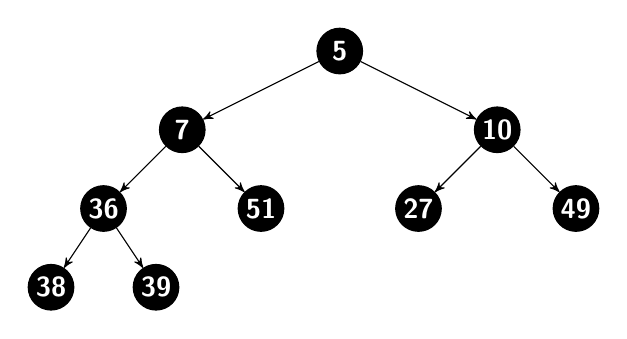
\begin{tikzpicture}[->,>=stealth',level/.style={sibling distance = 4cm/#1,
                    level distance = 1cm}] 
                  \node [arn_n] {5}
                  child{ node [arn_n] {7}
                    child{ node [arn_n] {36} 
                      child{ node [arn_n] {38}}
                      child{ node [arn_n] {39}}
                    }
                    child{ node [arn_n] {51}
                  }
                }
                child{ node [arn_n] {10} 
                    child{ node [arn_n] {27} 
                    }
                    child{ node [arn_n] {49}}                             
                  }
                ; 
                \end{tikzpicture}
                \caption{Un tas, dont la racine a pour valeur $5$, son
                  fils gauche a une racine de valeur $7$ et son fils
                  droit a pour racine un n\oe ud dont la  valeur est 10. Les
                  arbres vides ne sont pas repr{\'e}sent{\'e}s.}
                \label{fig:arbre}
        \end{subfigure}%
        \qquad
        \begin{subfigure}[b]{0.4\textwidth}
                \centering
                %\small
                \begin{tabular}[c]{|c|c|c|c|c|c|c|c|c|c|c|c|}
                  \hline
                  5 & 7 & 10 & 36 & 51 & 27 & 49 & 38 & 39 &  &  &  \\
                  \hline
                  \multicolumn 2l{0} & \multicolumn 3l{2} &
                  \multicolumn 7l {5} \\
                \end{tabular}
                \vspace*{2em}
                \caption{Le tableau correspondant {\`a} ce tas: la valeur
                  de la racine est dans la case $0$, celle de son fils
                droit dans la case $2=2\times 0+2$, et celle du fils
                gauche de ce fils droit est dans la case $5=2\times 2
                + 1$.}
                \label{fig:tableau}
        \end{subfigure}
  \caption{Tas et leur repr{\'e}sentation par un tableau}
  \label{fig:graph}
\end{figure}

\begin{figure}
  \centering
          \begin{subfigure}[b]{0.45\textwidth}
                \centering
                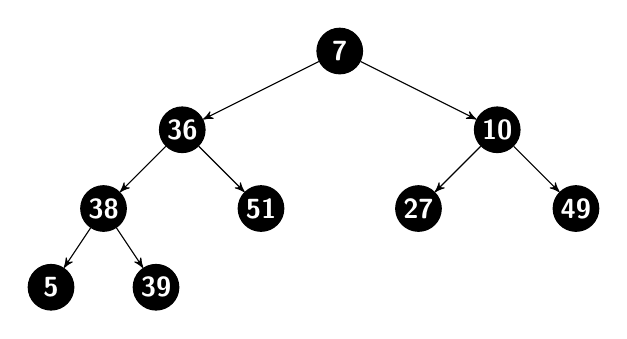
\begin{tikzpicture}[->,>=stealth',level/.style={sibling distance = 4cm/#1,
                    level distance = 1cm}] 
                  \node [arn_n] {7}
                  child{ node [arn_n] {36}
                    child{ node [arn_n] {38} 
                      child{ node [arn_n] {5}}
                      child{ node [arn_n] {39}}
                    }
                    child{ node [arn_n] {51}
                  }
                }
                child{ node [arn_n] {10} 
                    child{ node [arn_n] {27} 
                    }
                    child{ node [arn_n] {49}}                             
                  }
                ; 
                \end{tikzpicture}
                \caption{Le tas de la Figure~\ref{fig:arbre} apr{\`e}s
                  l'{\'e}tape 2 de la suppression.}
                \label{fig:tas:suppression:etape2}
        \end{subfigure}%
        \qquad
          \begin{subfigure}[b]{0.45\textwidth}
                \centering
                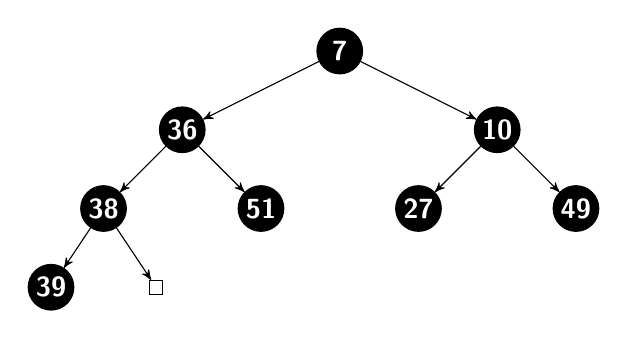
\begin{tikzpicture}[->,>=stealth',level/.style={sibling distance = 4cm/#1,
                    level distance = 1cm}] 
                  \node [arn_n] {7}
                  child{ node [arn_n] {36}
                    child{ node [arn_n] {38} 
                      child{ node [arn_n] {39}}
                      child{ node [arn_x] {}}
                    }
                    child{ node [arn_n] {51}
                  }
                }
                child{ node [arn_n] {10} 
                    child{ node [arn_n] {27} 
                    }
                    child{ node [arn_n] {49}}                             
                  }
                ; 
                \end{tikzpicture}
                \caption{Le tas de la Figure~\ref{fig:arbre} apr{\`e}s
                  l'{\'e}tape 5 de la suppression. Le n\oe ud vide
                  repr{\'e}sente la d{\'e}cr{\'e}mentation du nombre
                  d'{\'e}l{\'e}ments. $39$ est plus grand que $38$, donc
                  l'{\'e}tape 6 ne fait rien}
                \label{fig:tas:suppression:etape2}
        \end{subfigure}%
  \caption{Tas aux diff{\'e}rentes {\'e}tapes de la suppression.}
  \label{fig:tas:suppression:fig}
\end{figure}

\question (0.5 + 0.5 + 1 = 2 pts) {\'E}crire trois fonctions
\cfun{fils\_gauche}, \cfun{fils\_droit}, et \cfun{pere} qui, en
fonction d'un indice $i$, calculent l'indice correspondant
respectivement au fils gauche, au fils droit, et au p{\`e}re du n\oe ud
dont la valeur est stock{\'e}e dans la case $i$. \emph{Par exemple,
  \cfun{pere}(5)=2, et \cfun{fils\_gauche}(2)=5.}

\question (1 pt) {\'E}crire une fonction qui prend en entr{\'e}e un nombre
maximal d'{\'e}l{\'e}ments pour un tas, et qui rend un tas contenant $0$
{\'e}l{\'e}ments mais \emph{pouvant} contenir ce nombre maximal d'{\'e}l{\'e}ments.

L'algorithme permettant d'ins{\'e}rer un {\'e}l{\'e}ment dans un tas est donn{\'e}
informellement dans la Figure~\ref{fig:tas:insertion}.
\begin{figure}
  \begin{subfigure}[t]{0.45\textwidth}
    \centering
    \fbox{\parbox{\textwidth}{\begin{enumerate}\setlength\itemsep {-3pt}
        \item On note $i$ l'indice courant. Au d{\'e}part, l'indice courant
          est l'indice de la premi{\`e}re case vide dans le
          tableau (dans la Figure~\ref{fig:tableau}, $i$ vaut au d{\'e}part $9$);
        \item mettre l'{\'e}l{\'e}ment {\`a} ajouter dans la case d'indice $i$;
        \item Tant que:
          \begin{itemize}\setlength\itemsep {-3pt}
          \item l'indice courant est strictement positif;
          \item et la valeur du p{\`e}re de l'indice courant est plus grande que
            la valeur de l'indice courant
          \end{itemize}
          {\'e}changer ces deux valeurs, et positionner l'indice courant sur son
          p{\`e}re;
        \item rendre le tas;
        \end{enumerate}}\quad}
    \caption{Algorithme d'insertion d'un {\'e}l{\'e}ment.}
    \label{fig:tas:insertion}
  \end{subfigure}
  \qquad
  \begin{subfigure}[t]{0.45\textwidth}
    \centering
    \fbox{\parbox{\textwidth}{\begin{enumerate}\setlength\itemsep {-3pt}
        \item On note $i$ l'indice courant. Au d{\'e}part, l'indice courant
          vaut $0$;
        \item Tant que le fils droit de l'indice courant est dans le
          tableau:
          \begin{itemize}
          \item {\'e}changer la valeur du n\oe ud courant avec celle du plus
            petit de ses fils;
          \item l'indice courant devient celui du fils avec lequel
            l'{\'e}change a {\'e}t{\'e} fait.
          \end{itemize}
        \item Si l'{\'e}l{\'e}ment courant a un fils gauche, on {\'e}change ces deux
          {\'e}l{\'e}ments, et l'{\'e}l{\'e}ment courant devient l'indice du fils gauche;
        \item on {\'e}change ensuite la valeur de l'{\'e}l{\'e}ment courant et celle
          du dernier {\'e}l{\'e}ment du tas;
        \item on d{\'e}cr{\'e}mente de $1$ le nombre d'{\'e}l{\'e}ments dans le tas;
        \item on remonte, comme pour l'insertion, l'{\'e}l{\'e}ment courant tant
          qu'il est plus petit que son p{\`e}re.  
        \end{enumerate}}\quad}
    \caption{Algorithme de suppression du plus petit {\'e}l{\'e}ment.}
    \label{fig:tas:suppression}
  \end{subfigure}
  \label{fig:tas:algos}
  \caption{Algorithmes sur les tas}
\end{figure}

\question (1 pt) Justifiez (informellement) que l'insertion d'un
{\'e}l{\'e}ment dans un tas permet d'obtenir un tas, \textit{i.e.}, que dans
le tas obtenu, tout {\'e}l{\'e}ment est plus petit que ses fils.

\question (2 pts) {\'E}crire la fonction d'insertion d'un {\'e}l{\'e}ment en C. On suppose
qu'il y a strictement moins d'{\'e}l{\'e}ments dans le tas que le nombre
maximal qu'il ne peut en contenir.

\question (2 pts) {\'E}crire la fonction de suppression du plus petit
{\'e}l{\'e}ment en C en se basant sur l'algorithme de la
figure~\ref{fig:tas:suppression}. On suppose qu'il y a au moins un
{\'e}l{\'e}ment dans le tas.




\newpage

\exo{Algorithmique (7 pts)}

La bibliothèque universitaire a actuellement des difficultés à gérer
son stock car elle est très fréquentée en ce moment et ne dispose pas
d'un nombre suffisant d'employés. Vous décidez de l'aider en écrivant
un programme informatique permettant de soulager le travail des
employés.

\paragraph{Ce que doit faire votre programme:}
La bibliothèque possède \textit{nbLivres} livres indexés de 0 à
\(\text{\it nbLivres} - 1\). Chaque jour, un certain nombre de clients
demandent à emprunter des livres pour une certaine durée. Si le livre
est disponible, la requête du client est satisfaite, sinon le client
repart sans livre.

Votre programme doit d'abord lire sur une première ligne deux entiers:
\(\text{\it nbLivres} \le 10000\) et \textit{nbJours}. Pour chacun des
jours, votre programme lira un entier \textit{nbClients} sur une ligne puis
\textit{nbClients} lignes de deux entiers. Le premier entier correspond à
l'indice du livre et le second la durée correspondante. (voir
l'exemple d'entrée). Il affichera ensuite, sur des lignes séparées,
pour chaque client un 1 si le livre peut être prêté et 0 dans le cas
contraire.

On remarquera que si un client emprunte un livre le jour
\textit{iJour} pendant une durée \textit{duree} alors celui-ci ne sera
de nouveau disponible qu'au jour \(\text{\it iJour} + \text{\it
  duree}\). De plus, si plusieurs personnes demandent le même livre
pendant une journée, seule la première a une chance d'être satisfaite.

\paragraph{Exemple d'entrée.} Les lignes commen\c cant par \texttt{//}
sont des commentaires décrivant le contenu de la ligne suivante.

{\obeylines
\texttt{// nombre de livres}
10
\texttt{// nombre de jours à traiter}
2
\texttt{// nombre de clients le premier jour}
1
\texttt{// emprunt du livre 3 pour 2 jours}
3 2
\texttt{// nombre de clients le second jour}
2
\texttt{// emprunt du livre 3 pour 1 journée}
3 1
\texttt{// emprunt du livre 0 pour 2 jours}
0 2
}
Le programme doit afficher:
{\obeylines
\texttt{// premier emprunt accepté}
1
\texttt{// deuxième emprunt refusé car le livre a été prêté la veille}
0
\texttt{// troisième emprunt accepté}
1
}

\question (1 pt) Écrire une fonction qui lit le nombre de livres et
alloue un tableau contenant, pour chaque livre, le jour (un entier)
o\`u il sera livre. Initialement, aucun livre n'est emprunté.

\question (2 pts) Écrire une fonction qui prend entrée le tableau des
disponibilités, lit une ligne correspondant à un emprunt (2 entiers), et:
\begin{itemize}
\item affiche 0 si l'emprunt est refusé, et 1 s'il est accepté;
\item met à jour le tableau si l'emprunt est accepté.
\end{itemize}

\question (2 pts) Écrire une fonction qui prend entrée le tableau des
disponibilités, lit le nombre d'emprunts sur une journée, et met le
tableau à jour pour cette journée.

\question (2 pts) Écrire le programme résolvant le problème.




\newpage



\exo{Algorithmique (4 pts)}

Ecouter de la musique peut être très agréable mais lorsqu'un morceau
est vraiment très répétitif, il arrive parfois qu'on s'ennuie un
peu. Aussi le professeur de composition musicale du conservatoire a
décidé d'imposer une règle très stricte : quand il relit les morceaux
composés par ses élèves, dès qu'il voit deux notes identiques côte à
côte, il les efface toutes les deux ! Il continue ainsi d'effacer tant
qu'il existe deux notes égales consécutives.

Ce travail étant long et fastidieux, il se demande s'il n'est pas
possible de l'automatiser.


\question (4 pts) Écrire une fonction C prenant en argument une chaîne
de caractères représentant le morceau de musique (on supposera qu'elle
est correcte) et qui affiche version du morceau "corrigée" où tous les
doublons sont supprimés tant qu'il en existe. Les notes de musiques
sont représentées par les lettres 'a', 'b', 'c', 'd', 'e', 'f' et 'g'.


\newpage


\exo{Codage (4 points)}


\question Traduire les entiers 13 et -13 sur 5 bits en complément à deux.

\begin{solution}
  \begin{enumerate}
  \item On a \(2^5=32\), donc on peut coder les entiers de \(-16\) à
    \(+15\), et donc \(-13\) et \(13\);
  \item En complément à deux sur \(n\) bits, les entiers sont codés
    modulo \(2^n\), donc ici modulo \(32\)
  \item Comme entiers positifs, il faut donc trouver le codage de
    \(13\) et \(-13+32=19\).
  \item \(13=8+4+1=(1101)_2=01101\) sur 5 bits;
  \item \(19=16+2+1=(10011)_2=10011\) sur 5bits.
  \end{enumerate}

\end{solution}


\question Traduire si possible les entiers \(-8\), \(-7\), \(7\) et \(8\) sur 4
bits en complément à deux.

\begin{solution}
  \begin{enumerate}
  \item On a \(2^4=16\), donc on peut coder les entiers de \(-8\) à
    \(+7\), et donc seulement \(-8\), \(-7\) et \(7\);
  \item En complément à deux sur \(n\) bits, les entiers sont codés
    modulo \(2^n\), donc ici modulo \(16\)
  \item Comme entiers positifs, il faut donc trouver le codage de
    \(7\) et \(-8+16=8\) et \(-7+16 = 9\).
  \item \(7=4+2+1=(111)_2=0111\) sur 4 bits;
  \item \(8=8=(1000)_2=1000\) sur 4 bits;
  \item \(8=8+1=(1001)_2=1001\) sur 4 bits;
  \end{enumerate}

\end{solution}

\newpage

\exo{Conversion vers d'autres bases}

\question (2 pts) Traduire \(1,23\) en base 2 avec 10 chiffres
significatifs (en base 2).


\begin{solution}
  Pour avoir 10 chiffres en base 2, il en faut 3 en base 16 (et on
  aura une estimation trop précise ayant 12 chiffres en base 2):
  \begin{eqnarray*}
    0,23 \cdot 16 &=& \fbox{3},68\\
    0,68\cdot 16 &=& \fbox{10},88\\
    0,88\cdot 16 &=& \fbox{14},08\\
  \end{eqnarray*}
  Donc:
  \begin{eqnarray*}
    1,23 &=& (1,3AE)_{16}\\
    &=&(1,0011\,1010\,1110)_2\\
    &=&\fbox{\((1,0011\,1010\,11)_2\)}\hspace*{2em}\text{avec 10 chiffres significatifs}\\
  \end{eqnarray*}
  
\end{solution}

\question (2 pts) Traduire exactement \(1,25\) en base 2 et en base 16.


\begin{solution}
  On commence par la traduction en base 16:
  \begin{eqnarray*}
    0,25 \cdot 16 &=& \fbox{4},0\\
  \end{eqnarray*}
  Donc:
  \begin{eqnarray*}
    1,25 &=& (1,4)_{16}\\
    &=&(1,01)_2\\
  \end{eqnarray*}
  
\end{solution}


\question (2 pts) Traduire exactement \(44,125\) en base 2 et en base 16.


\begin{solution}
  On commence par la traduction en base 16:
  \begin{eqnarray*}
    0,125 \cdot 16 &=& \fbox{2},0\\
    44=2\cdot 16 + \underbrace{12}_{C}
  \end{eqnarray*}
  Donc:
  \begin{eqnarray*}
    44,125 &=& (2C,2)_{16}\\
    &=&(101100,0010)_2\\
  \end{eqnarray*}
  
\end{solution}



\newpage


On rappelle qu'un nombre:
\[
x=(-1)^s\cdot 2^{e-127}\cdot (1+\frac M{2^{23}})
\]
est codé sous la forme:
\begin{center}
  \begin{tabular}{|c|c|c|}
    \multicolumn 1c 0& \multicolumn 1c{\hbox to 8em{1\hfill 8}}&  \multicolumn 1c{\hbox to 23em {9\hfill 31}}\\
    \hline
    s &  e & M \\
    \hline
  \end{tabular}
\end{center}

\question (2 pts) Donnez le code hexadécimal du signe \(s\), de l'exposant \(e\), et de la mantisse \(M\), ainsi que le code entier sur 32 bits, du nombre \(-10,5\).

\begin{solution}
  On a:
  \begin{eqnarray*}
    -10,5&=&(-1)^1\cdot 2^3\cdot (1 + \frac{2,5}{8})\\
         &=& (-1)^1\cdot 2^{130-127}\cdot (1 + \frac{5}{16})\\
         &=& (-1)^1\cdot 2^{130-127}\cdot (1 + \frac{5}{2^4})\\
         &=& (-1)^1\cdot 2^{130-127}\cdot (1 + \frac{5\cdot 2^{19}}{2^{23}})\\
  \end{eqnarray*}
  Donc:
  \[
    s = 1 \hspace*{3em}e=130\hspace*{3em}M=5\cdot 2^{19}
  \]
  En base 16 (hexadécimal):
  Donc:
  \[
    s = 1 \hspace*{3em}e=128+2=82\hspace*{3em}M=5\cdot 8\cdot 2^{16}=280000
  \]
  Pour écrire en binaire le code entier, on écrit tout en base 2:
  \[
    \overbrace{\underbrace{1}_1}^s\,\,
    \overbrace{\underbrace{1000}_8\,\underbrace{0010}_2}^e\,\,
    \overbrace{\underbrace{010}_2\,\underbrace{1000}_8\,\underbrace{0000}_0\,\underbrace{0000}_0\,\underbrace{0000}_0\,\underbrace{0000}_0}^{M\text{ sur 23 bits}}
  \]
  et on regroupe par groupe de 4, qu'on traduit en hexadécimal:
  \[
    \underbrace{1100}_{12=C}\,\underbrace{0001}_1\,\underbrace{0010}_2\,\underbrace{1000}_8\,\underbrace{0000}_0\,\underbrace{0000}_0\,\underbrace{0000}_0\,\underbrace{0000}_0
  \]
  Donc le code entier en hexadécimal est \(C1280000\).
\end{solution}

\question (2 pts) Donnez le code hexadécimal du signe \(s\), de l'exposant \(e\), et de la mantisse \(M\), ainsi que le code entier sur 32 bits, du nombre \(3,25\).

\question (2 pts) Donnez le code hexadécimal du signe \(s\), de l'exposant \(e\), et de la mantisse \(M\), ainsi que le code entier sur 32 bits, du nombre \(-3,875\).


\newpage

\exo{Test de compréhension (4 points)}

\begin{center}
  \fbox{~\parbox{0.9\textwidth}{%
      Comme cela n'a pas été beaucoup vu en TP, on rappelle que si \(x\) est une valeur, alors:
      \begin{center}
        \texttt{( t ) x}
      \end{center}
      est la traduction de cette valeur dans le type \texttt{t}.
    }~}
\end{center}

On considère la fonction \texttt{main} suivante:

\begin{lstlisting}[language=C]
int main ( int argc , char * argv[] )
{
  int t[3] = {1,2,3} ;
  int * p1 = ( int * ) ( t + 1 ) ;
  int * p2 = ( int * ) ( & t + 1 ) - 1 ;
  * ( t + 2 ) = p1 [ 1 ] - t [ 0 ] ;
  p2[-2] = p1[1] ;
  printf ( "%d %d %d\n" , t[0] , t[1] , t[2] ) ;
  return 0 ;
}
\end{lstlisting}

\question (2 points) Expliquez, en vous aidant si possible de schémas,
quelles sont les valeurs, en tant qu'entier, de \(p_1\) et \(p_2\) en
fonction de la valeur de \(t\) en tant qu'entier. Pour simplifier, on
suppose que \texttt{sizeof ( int ) = 4}.
\begin{solution}
  Il est nécessaire (et suffisant) de faire un schéma de la mémoire pour s'y retrouver !
  Au début, on a:
  \begin{center}
    \begin{tabular}{|c|c|c|c|c|}
      \multicolumn 1l{100}&\multicolumn 1l{104}&\multicolumn 1l{108}&\multicolumn 1l{112}&\multicolumn 1l{116}\\
      \hline
      1&2&3&& \\
      \hline
      \multicolumn 1c{t[0]}&\multicolumn 1c{t[1]}&\multicolumn 1l{t[2]}&\multicolumn 1l{p1}&\multicolumn 1l{p2}\\
      \multicolumn 3c{\upbracefill}&\multicolumn 2c{}\\
      \multicolumn 3c{t}&\multicolumn 2c{}\\
    \end{tabular}
  \end{center}
  Pour les additions et soustractions sur les adresses en tant
  qu'entier, si \(x\) est l'adresse d'une valeur de type \texttt{t}, alors
  en tant qu'entier, \(x+1\) vaut \texttt{x + sizeof ( t )}.
  \begin{enumerate}
  \item \texttt{t} est l'adresse de \texttt{t[0]}, une valeur de type
    \texttt{int}, donc \texttt{t+1} vaut en tant qu'entier \texttt{t +
      sizeof ( int )}, soit \texttt{104} sur le schéma (c'est défini
    ainsi pour que \texttt{t+1} soit l'adresse de \texttt{t[1]});
  \item \texttt{\& t} est l'adresse de \texttt{t}, une
    valeur qui est un tableau de 3 entiers, donc
    \texttt{\& t+1} vaut en tant qu'entier \texttt{t + 3 *
      sizeof ( int )}, soit \texttt{112} sur le schéma. On traduit
    ensuite cette valeur en tant qu'adresse d'un entier, et on enlève 1, donc en tant qu'entier on obtient l'adresse \texttt{112 - sizeof ( int )=108}.
  \end{enumerate}
  Donc après l'initialisation, on a:
  \begin{center}
    \begin{tabular}{|c|c|c|c|c|}
      \multicolumn 1l{100}&\multicolumn 1l{104}&\multicolumn 1l{108}&\multicolumn 1l{112}&\multicolumn 1l{116}\\
      \hline
      1&2&3&104&108 \\
      \hline
      \multicolumn 1c{t[0]}&\multicolumn 1c{t[1]}&\multicolumn 1l{t[2]}&\multicolumn 1l{p1}&\multicolumn 1l{p2}\\
      \multicolumn 3c{\upbracefill}&\multicolumn 2c{}\\
      \multicolumn 3c{t}&\multicolumn 2c{}\\
    \end{tabular}
  \end{center}
  On passe ensuite à l'évaluation des 2 instructions:
  \begin{itemize}
  \item \texttt{t[2] = * ( p1 + 1 ) - t[0]}. D'après ce qui précède,
    \texttt{p1+1} est l'adresse de \texttt{t[2]}, donc on pourrait
    écrire de manière plus simple: \texttt{t[2] = t[2] - t[0]=2};
  \item \texttt{p2[-2] = t[2]}. D'après ce qui précède, \texttt{p2-2}
    est l'adresse d'une case contenant un entier 2 cases contenant des
    entiers avant \texttt{t[2]}, donc on pourrait écrire de manière
    plus simple: \texttt{t[0] = t[2] =2};
  \end{itemize}
  Donc avant le \texttt{printf}, le contenu de la mémoire est:
  \begin{center}
    \begin{tabular}{|c|c|c|c|c|}
      \multicolumn 1l{100}&\multicolumn 1l{104}&\multicolumn 1l{108}&\multicolumn 1l{112}&\multicolumn 1l{116}\\
      \hline
      2&2&2&104&108 \\
      \hline
      \multicolumn 1c{t[0]}&\multicolumn 1c{t[1]}&\multicolumn 1l{t[2]}&\multicolumn 1l{p1}&\multicolumn 1l{p2}\\
      \multicolumn 3c{\upbracefill}&\multicolumn 2c{}\\
      \multicolumn 3c{t}&\multicolumn 2c{}\\
    \end{tabular}
  \end{center}  
  Le programme affiche \texttt{2 2 2}.

   
\end{solution}


\newpage

\exo{Compréhension}

\begin{lstlisting}[language=C]
#include <stdio.h>

int
main ( int argc , char * argv[] )
{
  int x[3] ;
  printf ( "l'adresse de x[0] est %p.\n" , & x[0] ) ;
  printf ( "l'adresse de x[1] est %p.\n" , & x[1] ) ;
  printf ( "l'adresse de x[2] est %p.\n" , & x[2] ) ;
  printf ( "la valeur de x est %p.\n" , x ) ;
  printf ( "l'adresse de x est %p.\n" , & x ) ;
  printf ( "& x[1] - & x[0] = %ld\n" , & x[1] - & x[0] ) ;
  printf ( "& x[2] - & x[1] = %ld\n" , & x[2] - & x[1] ) ;
  printf ( "& x[2] - & x[0 = %ld\n" , & x[2] - & x[0] ) ;
  * ( & x[0] - 2 ) = 0 ;
  * ( & x[0] + 1 ) = 1 ;
  * ( & x[0] + 2 ) = 2 ;
  * ( & x[0] + 3 ) = 3 ;
  printf ( "x[0] = %d, x[1] = %d, x[2] = %d\n" , x[0] , x[1] , x[2] ) ;
  printf ( "sizeof ( x ) = %ld\n" , sizeof ( x ) ) ;
  printf ( "sizeof ( & x ) = %ld\n" , sizeof ( & x ) ) ;
  return 0 ;
}    
\end{lstlisting}

\question Dire ce qui sera affiché quand il est possible de le
déterminer, et quels sont les liens avec les autres valeurs quand on
peut seulement relier des valeurs entre elles (par exemple, savoir que
\(x = y\) même si on ne connaît pas la valeur de \(x\)).


\newpage
\end{document}

